\documentclass[10pt]{beamer}
\usetheme[
%%% options passed to the outer theme
%    hidetitle,           % hide the (short) title in the sidebar
%    hideauthor,          % hide the (short) author in the sidebar
%    hideinstitute,       % hide the (short) institute in the bottom of the sidebar
%    shownavsym,          % show the navigation symbols
%    width=2cm,           % width of the sidebar (default is 2 cm)
hideothersubsections,% hide all subsections but the subsections in the current section
%    hideallsubsections,  % hide all subsections
    left               % right of left position of sidebar (default is right)
%%% options passed to the color theme 
%    lightheaderbg,       % use a light header background
  ]{AAUsidebar}

% If you want to change the colors of the various elements in the theme, edit and uncomment the following lines
% Change the bar and sidebar colors:
%\setbeamercolor{AAUsidebar}{fg=red!20,bg=red}
%\setbeamercolor{sidebar}{bg=red!20}
% Change the color of the structural elements:
%\setbeamercolor{structure}{fg=red}
% Change the frame title text color:
%\setbeamercolor{frametitle}{fg=blue}
% Change the normal text color background:
%\setbeamercolor{normal text}{bg=gray!10}
% ... and you can of course change a lot more - see the beamer user manual.

\usepackage{pifont}
\usepackage[utf8]{inputenc}
\usepackage[english]{babel}
\usepackage[T1]{fontenc}
% Or whatever. Note that the encoding and the font should match. If T1
% does not look nice, try deleting the line with the fontenc.
\usepackage{helvet}
\usepackage{wasysym}
\usepackage[export]{adjustbox}
% colored hyperlinks
\newcommand{\chref}[2]{%
  \href{#1}{{\usebeamercolor[bg]{AAUsidebar}#2}}%
}



\usepackage{pgfplots}
\pgfplotsset{filter discard warning = true, unbounded coords=discard}
\pgfplotsset{compat = newest}


\title[]% optional, use only with long paper titles
{Development of a Simple Near-Ground Path Loss Model Verified by Measurements\\}

\subtitle{SEMCON 2016}  % could also be a conference name



\author[] % optional, use only with lots of authors
{
Mads Gotthardsen and Thomas Jørgensen
  %Group 16gr651
  %\href{mailto:jkn@es.aau.dk}{{\tt jkn@es.aau.dk}}
}

\date{December 22, 2016}
% - Give the names in the same order as they appear in the paper.
% - Use the \inst{?} command only if the authors have different
%   affiliation. See the beamer manual for an example

\institute[
%  {\includegraphics[scale=0.2]{aau_segl}}\\ %insert a company, department or university logo
  16gr751\\
  1st Semester WCS
] % optional - is placed in the bottom of the sidebar on every slide
{% is placed on the title page
  16gr751\\
  1st Semester WCS
  
  %there must be an empty line above this line - otherwise some unwanted space is added between the university and the country (I do not know why;( )
}


% specify a logo on the titlepage (you can specify additional logos an include them in 
% institute command below
%\pgfdeclareimage[width=5 cm]{titlepagelogo}{AAUgraphics/frontpageCropped.png} % placed on the title page
%\pgfdeclareimage[height=1.5cm]{titlepagelogo}{AAUgraphics/aau_logo_newOLD}
%\pgfdeclareimage[height=1.5cm]{titlepagelogo2}{graphics/aau_logo_new} % placed on the title page
\titlegraphic{% is placed on the bottom of the title page
 			 %\pgfuseimage{titlepagelogo}
             
\includegraphics[width = 0.2\textwidth]{AAUgraphics/aau_logo_newOLD.pdf}
%  \hspace{1cm}\pgfuseimage{titlepagelogo2}
}

\usepackage{tikz}
\usepackage[framemethod=tikz]{mdframed}
\usepackage[americanresistors,americaninductors,americancurrents, americanvoltages]{circuitikz}

\newmdenv[tikzsetting={draw=black,fill=white,fill opacity=0.7, line width=4pt},backgroundcolor=none,leftmargin=0,rightmargin=0,innertopmargin=0pt,skipbelow=\baselineskip,%
skipabove=\baselineskip]{TitleBox}


\definecolor{blockcolor}{RGB}{112,168,218}

\tikzstyle{blockbig} = [draw, fill=blockcolor, rectangle, 
    minimum height=3em, minimum width=6em]
\tikzstyle{block} = [draw, fill=blockcolor, rectangle, 
    minimum height=2em, minimum width=2em]
    
\tikzstyle{blockbigclear} = [draw, fill=white, rectangle, 
    minimum height=3em, minimum width=6em]
\tikzstyle{blockclear} = [draw, fill=white, rectangle, 
    minimum height=2em, minimum width=2em]
    
\tikzstyle{sum} = [draw, fill=blockcolor, circle, node distance=1.5cm, minimum size=0.6cm]
\tikzstyle{sumclear} = [draw, fill=white, circle, node distance=1.5cm, minimum size=0.6cm]
\tikzstyle{input} = [coordinate]
\tikzstyle{output} = [coordinate]
\tikzstyle{pinstyle} = [pin edge={to-,thin,black}]

\definecolor{thomasred}{RGB}{247,73,15} %217
\definecolor{thomasblue}{RGB}{0,114,189}
\definecolor{thomasyellow}{RGB}{237,179,32}
\definecolor{thomaspurple}{RGB}{126,47,142}
\definecolor{thomasgreen}{RGB}{119,172,48}
\usepackage{colortbl}

%%%%%%%%%%%%%%%%%%%%%%%%%%%%%%%%%%%%%%%%%%%%%%%%%%
\begin{document}
\setbeamertemplate{caption}{\raggedright\insertcaption\par}
% the titlepage
 {\aauwavesbg%  
%\usebackgroundtemplate{\includegraphics[width=\paperwidth]{frontpage.pdf}}
\begin{frame}[plain,noframenumbering] % the plain option removes the sidebar and header from the title page
\maketitle
%    \begin{figure}[!htbp]
%    \centering
%    \includegraphics[width=0.8\textwidth]{frontpageCropped.png}
%    \end{figure}
\end{frame}}

%%%%%%%%%%%%%%%%%%%%%%%%%%%%%%%%%%%%%%%%%
\section{Introduction}
\begin{frame}{Introduction}
\begin{minipage}{0.5\textwidth}
\begin{itemize}
\item Wireless Sensor Networks
\begin{itemize}
\item Commercial
\item Military
\end{itemize}
\item Focus
\begin{itemize}
\item Accuracy
\item Applicability
\item Simplicity
\end{itemize}
\end{itemize}
\end{minipage}
\begin{minipage}{0.45\textwidth}
\begin{figure}[!htbp]
 \centering
  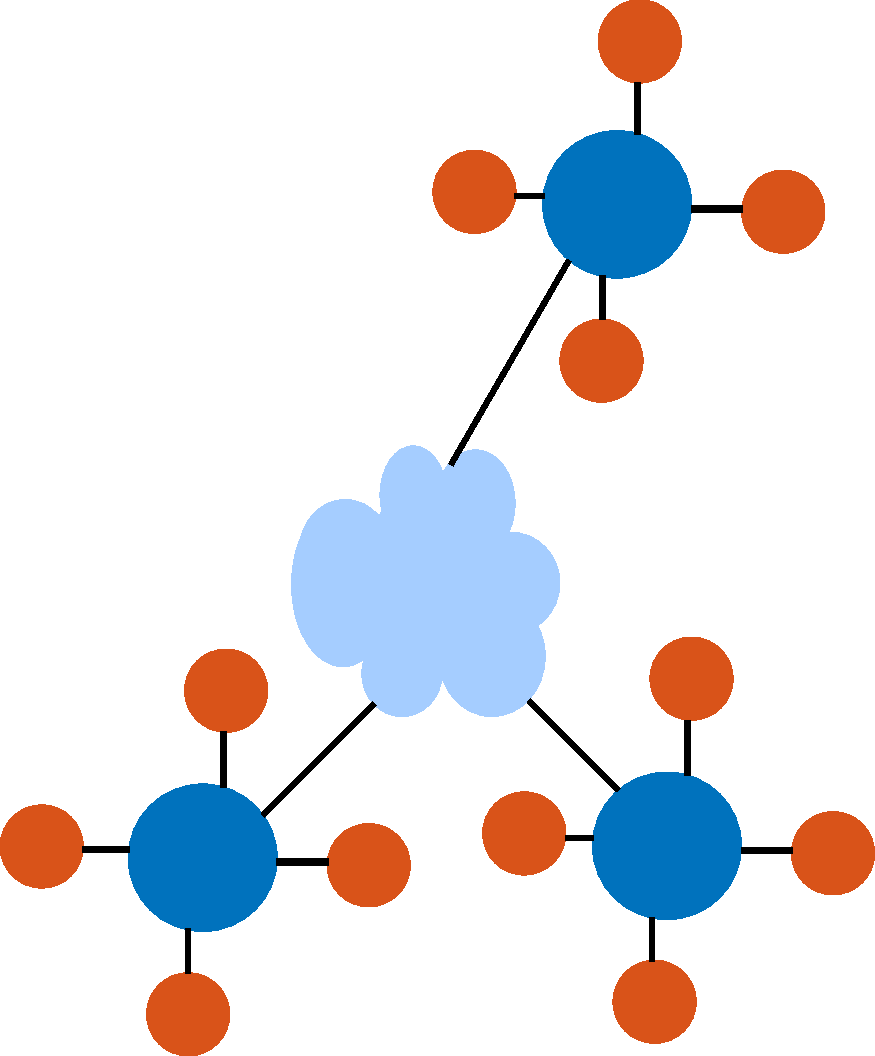
\includegraphics[width = \columnwidth]{figures/wsn_ill.pdf}
  \end{figure}
\end{minipage}
\end{frame}
 
%%%%%%%%%%%%%%%%%%%%%%%%%%%%%%%%%%%%%%%
\section{PL models}
\begin{frame}{PL models}
\begin{minipage}{.45\textwidth}
\raggedright\textcolor{thomasblue}{\textbf{Friss free space PL (FSPL)}:}
\begin{itemize}
\item Only direct wave
\item High heights
\end{itemize} 

\vspace{1em}
\textcolor{black}{\textbf{Conditions:}}
\begin{itemize}
\item No Multipath
\item $d >> \lambda$
\end{itemize}
\end{minipage}
\begin{minipage}{0.5\textwidth}

\begin{figure}[!htbp]
 \centering
  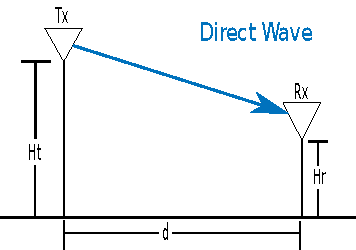
\includegraphics[width = \columnwidth]{figures/friss_illu.pdf}
  \end{figure}
\end{minipage}

\vspace{1em}
\begin{equation*}
L_p=\left(\frac{4 \pi d}{\lambda}\right)^2
\end{equation*}
\end{frame}


\begin{frame}{PL models}
\begin{minipage}{.45\textwidth}
\raggedright\textcolor{thomasred}{\textbf{Approximated two-ray}}\\
\raggedright\textcolor{thomasred}{\textbf{ground-reflection PL (ATRPL)}:}
\begin{itemize}
\item Direct and reflected wave
\item Medium heights
\end{itemize} 

\vspace{1em}
\textcolor{black}{\textbf{Conditions:}}
\begin{itemize}
\item No obstacles
\item Plane surface
\item $d > \frac{4\pi \cdot h_t h_r }{\lambda}$
\end{itemize}

\end{minipage}
\begin{minipage}{0.5\textwidth}
\begin{figure}[!htbp]
 \centering
  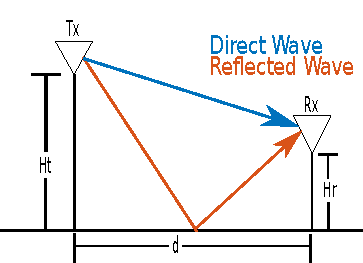
\includegraphics[width = \columnwidth]{figures/two_ray_illu.pdf}
  \end{figure}
\end{minipage}

\vspace{1em}
\begin{equation*}
L_{p} = \left(\frac{d^2}{h_t h_r}\right)^2
\label{two_ray_model}
\end{equation*}
\end{frame}


\begin{frame}{PL models}
\begin{minipage}{.45\textwidth}
\raggedright\textcolor{thomasgreen}{\textbf{Norton surface wave PL (NSPL)}:}
\begin{itemize}
\item Only surface wave
\item Low heights
\item Dependent on surface constants
\end{itemize}

\vspace{1em}
\textcolor{black}{\textbf{Conditions:}}
\begin{itemize}
\item No obstacles
\item Plane surface
\item $h_t,h_r > \lambda$
\end{itemize}

\end{minipage}%
\begin{minipage}{0.5\textwidth}
\begin{figure}[!htbp]
 \centering
  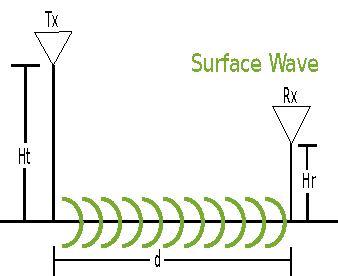
\includegraphics[width = \columnwidth]{figures/surf_illu.pdf}
  \end{figure}
\end{minipage}

\vspace{1em}
\begin{equation}
L_p=\left({d} \cdot \left|\frac{\lambda}{2\pi z}\right|^{-1}\right)^4
\label{surface_wave}
\end{equation}
\end{frame}



\begin{frame}{PL models}
\begin{minipage}{.45\textwidth}
\raggedright\textcolor{thomaspurple}{\textbf{Ground wave PL (GWPL)}:}
\begin{itemize}
\item All waves
\item All heights
\item Dependent on surface constants
\end{itemize} 

\vspace{1em}
\textcolor{black}{\textbf{Conditions:}}
\begin{itemize}
\item No obstacles
\item Plane surface
\end{itemize}

\end{minipage}
\begin{minipage}{0.5\textwidth}
\begin{figure}[!htbp]
 \centering
  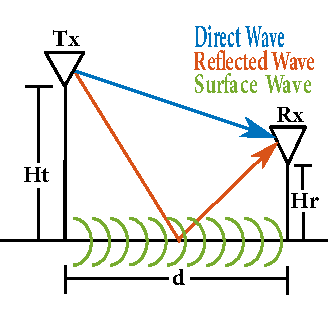
\includegraphics[width = \columnwidth]{figures/poster_cropped_1.pdf}
  \end{figure}
\end{minipage}

\vspace{1em}
\begin{equation}
L_p=\left(\frac{4 \pi d}{\lambda}\right)^2 \cdot \Big|\underbrace{1}_{\begin{subarray}{c}Direct\\wave\end{subarray}}+\underbrace{R\text{e}^{j\Delta}}_{\begin{subarray}{c}Reflected\\wave\end{subarray}}+\underbrace{(1-R)A\text{e}^{j\Delta}}_{\begin{subarray}{c}Surface\\wave\end{subarray}}\Big|^{-2} 
\label{ground_wave}
\end{equation}
\end{frame}

%%%%%%%%%%%%%%%%%%%%%%%%%%%%%%%%%%%%

\section{Measurements}
\begin{frame}{Measurements}
\begin{figure}[!htbp]
	\centering
	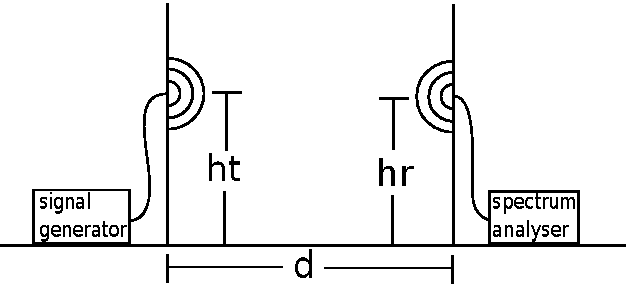
\includegraphics[width = \columnwidth]{figures/setup.pdf}
\end{figure}
\begin{minipage}{0.15\textwidth}
 \textcolor{white}{.}  
\end{minipage}%
\begin{minipage}{0.8\textwidth}
\begin{itemize}
\item 1 Frequency (858 MHz)
\item 2 Antenna sets (monopole and patch)
\item 2 Polarization (horizontal and vertical)
\item 2 Location (outdoor and indoor)
\item 4 Rx/Tx heights (from 0.04 to 2.02 m)
\item 6 Distances (from 1 to 30 m)
\end{itemize}
\end{minipage}
\end{frame}

%%%%%%%%%%%%%%%%%%%%%%%%%%%%%%%%%%%%%%%%%%%%
\definecolor{grey}{RGB}{230,230,230}
\section{Influence of parameters}
\begin{frame}{Influence of parameters}
\begin{table}[!htbp]
\footnotesize
\centering
\textcolor{black}{
\begin{tabular}{|c|c|c|c|}
\hline \rowcolor{black}
\textcolor{white}{Distance}    & \textcolor{white}{1 m} & \textcolor{white}{2 m}& \textcolor{white}{4 m}\\\hline\rowcolor{grey}
PL & (34.7$\pm 1.6$) dB & (41.4$\pm 1.4$) dB & (49.0$\pm 1.7$) dB  \\\hline
\multicolumn{4}{c}{}\\\hline\rowcolor{black}
\textcolor{white}{Distance}	&\textcolor{white}{8 m}& \textcolor{white}{15 m}& \textcolor{white}{30 m}\\\hline\rowcolor{grey}
PL &	(57.3$\pm 2.1$) dB & (66.1$\pm 2.5$) dB & (72.3$\pm 2.3$) dB \\\hline
\end{tabular}}
\end{table}
\begin{table}[H]
\centering
\resizebox{\linewidth}{!}{
\textcolor{black}{
\begin{tabular}{|c|c|c|c|c|}
\hline\rowcolor{black}
\textcolor{white}{h$_t$ \textbackslash h$_r$} &\textcolor{white}{ 0.04 m} & \textcolor{white}{0.14 m} &\textcolor{white}{ 0.36 m} &\textcolor{white}{ 2.02 m} \\\hline\rowcolor{grey}
\cellcolor{black}\textcolor{white}{0.04 m} & (63.7$\pm 5.2$) dB & (60.7$\pm 5.1$) dB & (55.4$\pm 4.7$) dB & (52.4$\pm 3.8$) dB\\\hline
\cellcolor{black}\textcolor{white}{0.14 m} & (60.7$\pm 5.1$) dB & (58.1$\pm 5.2$) dB & (53.4$\pm 4.5$) dB & (50.2$\pm 3.2$) dB\\\hline\rowcolor{grey}
\cellcolor{black}\textcolor{white}{0.36 m} & (55.4$\pm 4.7$) dB & (53.4$\pm 4.5$) dB & (49.0$\pm 2.9$) dB & (47.6$\pm 4.8$) dB\\\hline
\cellcolor{black}\textcolor{white}{2.02 m} & (52.4$\pm 3.8$) dB & (50.2$\pm 3.2$) dB & (47.6$\pm 4.8$) dB & (44.4$\pm 3.1$) dB\\\hline
\end{tabular}}}
\end{table}

\begin{table}[H]
\textcolor{black}{
\resizebox{0.45\linewidth}{!}{
\begin{tabular}{|c|c|}\hline \rowcolor{black}
\textcolor{white}{Gym} &  \textcolor{white}{Parking lot}  \\\hline\rowcolor{grey}
(52.4$\pm 1.8$) dB& (54.6$\pm 2.2$) dB \\\hline
\end{tabular}}
\resizebox{0.45\linewidth}{!}{
\begin{tabular}{|c|c|}\hline \rowcolor{black}
\textcolor{white}{Monopole} & \textcolor{white}{Patch}  \\\hline\rowcolor{grey}
(55.6$\pm 2.0$) dB & (51.4$\pm 2.0$) dB  \\\hline
\end{tabular}}}

\vspace{1em}
\textcolor{black}{
\resizebox{0.45\linewidth}{!}{
\begin{tabular}{|c|c|}\hline \rowcolor{black}
\textcolor{white}{Vertical} & \textcolor{white}{Horizontal} \\\hline\rowcolor{grey}
(51.8$\pm 1.9$) dB & (55.1$\pm 2.1$) dB \\\hline
\end{tabular}}}
\end{table}
\end{frame}

%%%%%%%%%%%%%%%%%%%%%%%%%%%%%%%%%%%%%%%%%%%%%%%
\section{Proposed PL model}
\begin{frame}{Proposed PL model}
%\begin{equation*}
%ATRPL = \left(\frac{d^2}{h_t h_r}\right)^2
%\label{two_ray_model}
%\end{equation*}
%
%\begin{equation*}
%d > \frac{4\pi \cdot h_t h_r }{\lambda}
%\label{two_ray_cond}
%\end{equation*}
%
%\begin{equation*}
%NSPL=\left(\frac{d}{h_{0}}\right)^4
%\label{surface_wave}
%\end{equation*}
\begin{minipage}{0.45\textwidth}
\resizebox{\textwidth}{!}{
% This file was created by matlab2tikz.
%
%The latest updates can be retrieved from
%  http://www.mathworks.com/matlabcentral/fileexchange/22022-matlab2tikz-matlab2tikz
%where you can also make suggestions and rate matlab2tikz.
%
\definecolor{mycolor1}{rgb}{0.00000,0.44700,0.74100}%
\definecolor{mycolor2}{rgb}{0.85000,0.32500,0.09800}%
\definecolor{mycolor3}{rgb}{0.92900,0.69400,0.12500}%
\definecolor{mycolor4}{rgb}{0.49400,0.18400,0.55600}%
\definecolor{mycolor5}{rgb}{0.46600,0.67400,0.18800}%
%
\begin{tikzpicture}

\begin{axis}[%
width=2.8in,
height=\myvar,
at={(0.758in,0.481in)},
scale only axis,
xmode=log,
extra x ticks={2,5,20}, 
extra x tick style={log identify minor tick positions=false},
log ticks with fixed point,
xmin=0.9,
xmax=31,
xlabel=Distance (m),
xminorticks=true,
xmajorgrids,
xminorgrids,
ymin=20,
ymax=100,
ylabel=Path loss (dB),
ymajorgrids,
axis background/.style={fill=white},
title style={font=\bfseries},
legend style={legend cell align=left,align=left,draw=white!15!black},
legend pos = south east
]

\addplot [color=mycolor1,mark size=2.5pt,only marks,mark=asterisk,mark options={solid}]
  table[row sep=crcr]{%
1	39.176832441447\\
2	50.0236813268286\\
4	61.7627349006033\\
8	69.1568155321866\\
15	80.2784721484843\\
30	81.8463231335614\\
};
\addlegendentry{Measured PL};

\addplot [color=mycolor2,dashed]
  table[row sep=crcr]{%
1	31.1115179430228\\
1.29292929292929	33.3430134440292\\
1.58585858585859	35.1168070992565\\
1.87878787878788	36.5890729354301\\
2.17171717171717	37.8475832493839\\
2.46464646464646	38.9466105778464\\
2.75757575757576	39.9220669918869\\
3.05050505050505	40.7989529102148\\
3.34343434343434	41.5953739265862\\
3.63636363636364	42.3248640664175\\
3.92929292929293	42.9978060775859\\
4.22222222222222	43.6223396865725\\
4.51515151515152	44.2049645137105\\
4.80808080808081	44.7509531054816\\
5.1010101010101	45.264641613445\\
5.39393939393939	45.7496391916429\\
5.68686868686869	46.2089819480987\\
5.97979797979798	46.6452481855302\\
6.27272727272727	47.0606460546034\\
6.56565656565657	47.4570811839289\\
6.85858585858586	47.8362095366818\\
7.15151515151515	48.1994792048672\\
7.44444444444444	48.5481638082528\\
7.73737373737374	48.8833894437239\\
8.03030303030303	49.2061566242012\\
8.32323232323232	49.5173582850141\\
8.61616161616162	49.8177946744222\\
8.90909090909091	50.1081857537082\\
9.2020202020202	50.3891815905317\\
9.49494949494949	50.6613711230658\\
9.78787878787879	50.9252895920871\\
10.0808080808081	51.1814248768192\\
10.3737373737374	51.4302229230174\\
10.6666666666667	51.6720924150277\\
10.959595959596	51.9074088147627\\
11.2525252525253	52.136517867826\\
11.5454545454545	52.3597386589774\\
11.8383838383838	52.5773662847132\\
12.1313131313131	52.7896741991299\\
12.4242424242424	52.9969162798597\\
12.7171717171717	53.199328653229\\
13.010101010101	53.3971313115477\\
13.3030303030303	53.5905295503075\\
13.5959595959596	53.7797152488309\\
13.8888888888889	53.9648680143974\\
14.1818181818182	54.1461562069475\\
14.4747474747475	54.3237378590187\\
14.7676767676768	54.4977615035086\\
15.0606060606061	54.6683669201317\\
15.3535353535354	54.8356858099672\\
15.6464646464646	54.9998424062559\\
15.9393939393939	55.1609540285398\\
16.2323232323232	55.3191315863387\\
16.5252525252525	55.4744800377779\\
16.8181818181818	55.6270988079186\\
17.1111111111111	55.7770821709656\\
17.4040404040404	55.9245196000324\\
17.6969696969697	56.069496087713\\
17.989898989899	56.2120924403367\\
18.2828282828283	56.3523855484555\\
18.5757575757576	56.4904486358333\\
18.8686868686869	56.6263514889533\\
19.1616161616162	56.760160668845\\
19.4545454545455	56.8919397068421\\
19.7474747474747	57.0217492857095\\
20.040404040404	57.149647407435\\
20.3333333333333	57.2756895488449\\
20.6262626262626	57.3999288060896\\
20.9191919191919	57.5224160289408\\
21.2121212121212	57.6431999457502\\
21.5050505050505	57.7623272798382\\
21.7979797979798	57.8798428580096\\
22.0909090909091	57.9957897118245\\
22.3838383838384	58.1102091721996\\
22.6767676767677	58.2231409578586\\
22.969696969697	58.3346232581061\\
23.2626262626263	58.4446928103564\\
23.5555555555556	58.5533849728113\\
23.8484848484848	58.6607337926463\\
24.1414141414141	58.7667720700345\\
24.4343434343434	58.8715314183094\\
24.7272727272727	58.9750423205423\\
25.020202020202	59.0773341827885\\
25.3131313131313	59.1784353842344\\
25.6060606060606	59.2783733244589\\
25.8989898989899	59.3771744680074\\
26.1919191919192	59.4748643864588\\
26.4848484848485	59.5714677981531\\
26.7777777777778	59.6670086057337\\
27.0707070707071	59.7615099316476\\
27.3636363636364	59.8549941517351\\
27.6565656565657	59.9474829270312\\
27.9494949494949	60.0389972338908\\
28.2424242424242	60.1295573925447\\
28.5353535353535	60.2191830941809\\
28.8282828282828	60.3078934266443\\
29.1212121212121	60.3957068988359\\
29.4141414141414	60.4826414638918\\
29.7070707070707	60.5687145412132\\
30	60.653943037416\\
};
\addlegendentry{FSPL};

\addplot [color=mycolor3, solid]
  table[row sep=crcr]{%
1	54.6612617768166\\
1.29292929292929	59.1242527788293\\
1.58585858585859	62.6718400892839\\
1.87878787878788	65.6163717616312\\
2.17171717171717	68.1333923895388\\
2.46464646464646	70.3314470464637\\
2.75757575757576	72.2823598745448\\
3.05050505050505	74.0361317112006\\
3.34343434343434	75.6289737439433\\
3.63636363636364	77.087954023606\\
3.92929292929293	78.4338380459428\\
4.22222222222222	79.6829052639159\\
4.51515151515152	80.848154918192\\
4.80808080808081	81.9401321017343\\
5.1010101010101	82.967509117661\\
5.39393939393939	83.9375042740568\\
5.68686868686869	84.8561897869684\\
5.97979797979798	85.7287222618313\\
6.27272727272727	86.5595179999777\\
6.56565656565657	87.3523882586288\\
6.85858585858586	88.1106449641346\\
7.15151515151515	88.8371843005053\\
7.44444444444444	89.5345535072766\\
7.73737373737374	90.2050047782187\\
8.03030303030303	90.8505391391734\\
8.32323232323232	91.4729424607992\\
8.61616161616162	92.0738152396155\\
8.90909090909091	92.6545973981873\\
9.2020202020202	93.2165890718345\\
9.49494949494949	93.7609681369025\\
9.78787878787879	94.2888050749451\\
10.0808080808081	94.8010756444094\\
10.3737373737374	95.2986717368057\\
10.6666666666667	95.7824107208263\\
10.959595959596	96.2530435202965\\
11.2525252525253	96.7112616264229\\
11.5454545454545	97.1577032087258\\
11.8383838383838	97.5929584601974\\
12.1313131313131	98.0175742890308\\
12.4242424242424	98.4320584504904\\
12.7171717171717	98.8368831972291\\
13.010101010101	99.2324885138663\\
13.3030303030303	99.6192849913859\\
13.5959595959596	99.9976563884329\\
13.8888888888889	100.367961919566\\
14.1818181818182	100.730538304666\\
14.4747474747475	101.085701608808\\
14.7676767676768	101.433748897788\\
15.0606060606061	101.774959731034\\
15.3535353535354	102.109597510705\\
15.6464646464646	102.437910703283\\
15.9393939393939	102.760133947851\\
16.2323232323232	103.076489063448\\
16.5252525252525	103.387185966327\\
16.8181818181818	103.692423506608\\
17.1111111111111	103.992390232702\\
17.4040404040404	104.287265090836\\
17.6969696969697	104.577218066197\\
17.989898989899	104.862410771444\\
18.2828282828283	105.142996987682\\
18.5757575757576	105.419123162438\\
18.8686868686869	105.690928868678\\
19.1616161616162	105.958547228461\\
19.4545454545455	106.222105304455\\
19.7474747474747	106.48172446219\\
20.040404040404	106.737520705641\\
20.3333333333333	106.989604988461\\
20.6262626262626	107.23808350295\\
20.9191919191919	107.483057948653\\
21.2121212121212	107.724625782271\\
21.5050505050505	107.962880450447\\
21.7979797979798	108.19791160679\\
22.0909090909091	108.42980531442\\
22.3838383838384	108.65864423517\\
22.6767676767677	108.884507806488\\
22.969696969697	109.107472406983\\
23.2626262626263	109.327611511484\\
23.5555555555556	109.544995836394\\
23.8484848484848	109.759693476064\\
24.1414141414141	109.97177003084\\
24.4343434343434	110.18128872739\\
24.7272727272727	110.388310531855\\
25.020202020202	110.592894256348\\
25.3131313131313	110.79509665924\\
25.6060606060606	110.994972539689\\
25.8989898989899	111.192574826786\\
26.1919191919192	111.387954663689\\
26.4848484848485	111.581161487077\\
26.7777777777778	111.772243102238\\
27.0707070707071	111.961245754066\\
27.3636363636364	112.148214194241\\
27.6565656565657	112.333191744833\\
27.9494949494949	112.516220358553\\
28.2424242424242	112.69734067586\\
28.5353535353535	112.876592079133\\
28.8282828282828	113.05401274406\\
29.1212121212121	113.229639688443\\
29.4141414141414	113.403508818555\\
29.7070707070707	113.575654973197\\
30	113.746111965603\\
};
\addlegendentry{ATRPL};

\addplot [color=mycolor4,solid]
  table[row sep=crcr]{%
1	44.9214537765832\\
1.29292929292929	49.050887223414\\
1.58585858585859	52.3850957227753\\
1.87878787878788	55.1813933158306\\
2.17171717171717	57.5894450858098\\
2.46464646464646	59.7040212694623\\
2.75757575757576	61.5889394607992\\
3.05050505050505	63.2892290586399\\
3.34343434343434	64.8378512938563\\
3.63636363636364	66.2596600128227\\
3.92929292929293	67.5738601151063\\
4.22222222222222	68.7955994809671\\
4.51515151515152	69.9370368618302\\
4.80808080808081	71.0080800079665\\
5.1010101010101	72.0169091509038\\
5.39393939393939	72.970356641531\\
5.68686868686869	73.8741877133422\\
5.97979797979798	74.7333117479744\\
6.27272727272727	75.5519437159365\\
6.56565656565657	76.333729260202\\
6.85858585858586	77.0818428258175\\
7.15151515151515	77.7990655182941\\
7.44444444444444	78.4878475170174\\
7.73737373737374	79.1503585803853\\
8.03030303030303	79.7885292691858\\
8.32323232323232	80.4040848627714\\
8.61616161616162	80.9985734692596\\
8.90909090909091	81.5733894830492\\
9.2020202020202	82.1297932842206\\
9.49494949494949	82.668927879939\\
9.78787878787879	83.1918330403857\\
10.0808080808081	83.699457368673\\
10.3737373737374	84.1926686568157\\
10.6666666666667	84.6722628117708\\
10.959595959596	85.1389715821175\\
11.2525252525253	85.5934692737141\\
11.5454545454545	86.0363786090357\\
11.8383838383838	86.4682758579694\\
12.1313131313131	86.8896953461372\\
12.4242424242424	87.3011334292265\\
12.7171717171717	87.7030520074711\\
13.010101010101	88.0958816426928\\
13.3030303030303	88.4800243306433\\
13.5959595959596	88.8558559734019\\
13.8888888888889	89.223728589948\\
14.1818181818182	89.5839722974902\\
14.4747474747475	89.9368970915016\\
14.7676767676768	90.2827944485156\\
15.0606060606061	90.6219387724419\\
15.3535353535354	90.9545887023927\\
15.6464646464646	91.2809882976234\\
15.9393939393939	91.6013681131972\\
16.2323232323232	91.9159461782433\\
16.5252525252525	92.2249288872049\\
16.8181818181818	92.5285118132048\\
17.1111111111111	92.8268804515537\\
17.4040404040404	93.1202109004784\\
17.6969696969697	93.4086704853281\\
17.989898989899	93.6924183317962\\
18.2828282828283	93.9716058930773\\
18.5757575757576	94.2463774353278\\
18.8686868686869	94.5168704853298\\
19.1616161616162	94.7832162438333\\
19.4545454545455	95.0455399676875\\
19.7474747474747	95.3039613235475\\
20.040404040404	95.5585947156543\\
20.3333333333333	95.8095495899402\\
20.6262626262626	96.0569307164769\\
20.9191919191919	96.3008384520958\\
21.2121212121212	96.5413689848235\\
21.5050505050505	96.7786145616295\\
21.7979797979798	97.0126637008234\\
22.0909090909091	97.2436013903413\\
22.3838383838384	97.4715092730185\\
22.6767676767677	97.6964658198685\\
22.969696969697	97.9185464922848\\
23.2626262626263	98.1378238940042\\
23.5555555555556	98.3543679135994\\
23.8484848484848	98.5682458581985\\
24.1414141414141	98.7795225790731\\
24.4343434343434	98.9882605896812\\
24.7272727272727	99.1945201767008\\
25.020202020202	99.3983595045488\\
25.3131313131313	99.5998347138414\\
25.6060606060606	99.7990000142057\\
25.8989898989899	99.9959077718343\\
26.1919191919192	100.190608592132\\
26.4848484848485	100.383151397784\\
26.7777777777778	100.573583502539\\
27.0707070707071	100.761950681\\
27.3636363636364	100.948297234668\\
27.6565656565657	101.132666054478\\
27.9494949494949	101.315098680055\\
28.2424242424242	101.495635355893\\
28.5353535353535	101.674315084635\\
28.8282828282828	101.851175677652\\
29.1212121212121	102.02625380307\\
29.4141414141414	102.199585031394\\
29.7070707070707	102.371203878887\\
30	102.541143848821\\
};
\addlegendentry{GWPL};

\addplot [color=mycolor5,solid]
  table[row sep=crcr]{%
1	45.2757493241887\\
1.29292929292929	49.7228898745648\\
1.58585858585859	53.262521493136\\
1.87878787878788	56.2025058764576\\
2.17171717171717	58.7166869357065\\
2.46464646464646	60.912850849718\\
2.75757575757576	62.8624418401923\\
3.05050505050505	64.6152535121936\\
3.34343434343434	66.2073762348812\\
3.63636363636364	67.665803769948\\
3.92929292929293	69.0112538998\\
4.22222222222222	70.2599742986074\\
4.51515151515152	71.4249423794752\\
4.80808080808081	72.5166878414888\\
5.1010101010101	73.5438718794334\\
5.39393939393939	74.5137046228799\\
5.68686868686869	75.4322521586162\\
5.97979797979798	76.3046664254687\\
6.27272727272727	77.135360121141\\
6.56565656565657	77.9281416843724\\
6.85858585858586	78.6863208115117\\
7.15151515151515	79.41279190354\\
7.44444444444444	80.110100760591\\
7.73737373737374	80.7804984041527\\
8.03030303030303	81.4259848975564\\
8.32323232323232	82.0483453152401\\
8.61616161616162	82.6491794904726\\
8.90909090909091	83.2299267897558\\
9.2020202020202	83.7918868793997\\
9.49494949494949	84.3362372379378\\
9.78787878787879	84.864048007723\\
10.0808080808081	85.3762946565475\\
10.3737373737374	85.8738688257092\\
10.6666666666667	86.3575876675597\\
10.959595959596	86.8282019180994\\
11.2525252525253	87.2864029048315\\
11.5454545454545	87.7328286540697\\
11.8383838383838	88.1680692330933\\
12.1313131313131	88.5926714393722\\
12.4242424242424	89.0071429303434\\
12.7171717171717	89.4119558719659\\
13.010101010101	89.8075501718137\\
13.3030303030303	90.1943363522118\\
13.5959595959596	90.5726981104615\\
13.8888888888889	90.9429946061772\\
14.1818181818182	91.3055625099107\\
14.4747474747475	91.6607178423471\\
14.7676767676768	92.0087576292505\\
15.0606060606061	92.3499613938723\\
15.3535353535354	92.684592505612\\
15.6464646464646	93.0128994012286\\
15.9393939393939	93.3351166927899\\
16.2323232323232	93.651466174734\\
16.5252525252525	93.9621577408714\\
16.8181818181818	94.2673902208208\\
17.1111111111111	94.5673521442283\\
17.4040404040404	94.8622224401226\\
17.6969696969697	95.1521710779052\\
17.989898989899	95.4373596557222\\
18.2828282828283	95.717941941319\\
18.5757575757576	95.9940643699092\\
18.8686868686869	96.2658665030932\\
19.1616161616162	96.5334814524268\\
19.4545454545455	96.7970362708578\\
19.7474747474747	97.0566523149128\\
20.040404040404	97.3124455802169\\
20.3333333333333	97.5645270126694\\
20.6262626262626	97.8130027973644\\
20.9191919191919	98.0579746271396\\
21.2121212121212	98.2995399524521\\
21.5050505050505	98.5377922141197\\
21.7979797979798	98.7728210603168\\
22.0909090909091	99.0047125490867\\
22.3838383838384	99.233549337516\\
22.6767676767677	99.4594108586096\\
22.969696969697	99.6823734868158\\
23.2626262626263	99.9025106930627\\
23.5555555555556	100.119893190094\\
23.8484848484848	100.334589068825\\
24.1414141414141	100.546663926372\\
24.4343434343434	100.756180986366\\
24.7272727272727	100.963201212092\\
25.020202020202	101.167783412968\\
25.3131313131313	101.369984344831\\
25.6060606060606	101.569858804446\\
25.8989898989899	101.767459718646\\
26.1919191919192	101.962838228456\\
26.4848484848485	102.156043768541\\
26.7777777777778	102.347124142282\\
27.0707070707071	102.53612559277\\
27.3636363636364	102.72309286998\\
27.6565656565657	102.908069294363\\
27.9494949494949	103.091096817097\\
28.2424242424242	103.27221607719\\
28.5353535353535	103.451466455638\\
28.8282828282828	103.628886126821\\
29.1212121212121	103.804512107298\\
29.4141414141414	103.978380302156\\
29.7070707070707	104.150525549075\\
30	104.320981660217\\
};
\addlegendentry{NSPL};

\end{axis}
\end{tikzpicture}%
}
\end{minipage}%
\begin{minipage}{0.45\textwidth}
\resizebox{\textwidth}{!}{
% This file was created by matlab2tikz.
%
%The latest updates can be retrieved from
%  http://www.mathworks.com/matlabcentral/fileexchange/22022matlab2tikzmatlab2tikz
%where you can also make suggestions and rate matlab2tikz.
%
\definecolor{mycolor1}{rgb}{0.00000,0.44700,0.74100}%
\definecolor{mycolor2}{rgb}{0.85000,0.32500,0.09800}%
\definecolor{mycolor3}{rgb}{0.92900,0.69400,0.12500}%
\definecolor{mycolor4}{rgb}{0.49400,0.18400,0.55600}%
\definecolor{mycolor5}{rgb}{0.46600,0.67400,0.18800}%
%
\begin{tikzpicture}

\begin{axis}[%
width=2.8in,
height=\myvar,
at={(0.758in,0.481in)},
scale only axis,
xmode=log,
extra x ticks={2,5,20}, 
extra x tick style={log identify minor tick positions=false},
log ticks with fixed point,
xmin=0.9,
xmax=31,
xlabel=Distance (m),
xminorticks=true,
xmajorgrids,
xminorgrids,
ymin=20,
ymax=100,
ylabel=Path loss (dB),
ymajorgrids,
axis background/.style={fill=white},
legend style={legend cell align=left,align=left,draw=white!15!black},
legend pos = north west
]
\addplot [color=mycolor1,mark size=2.5pt,only marks,mark=asterisk,mark options={solid}]
  table[row sep=crcr]{%
1.03029316216308	31.28383923555\\
2.01531734473755	39.0242931377669\\
4.00768062599803	49.7368915447371\\
8.00384307692249	59.2686962142928\\
15.0020499932509	68.2995914203388\\
30.0010250491546	72.5078313840168\\
};
\addlegendentry{Measured PL};

\addplot [color=mycolor2,solid]
  table[row sep=crcr]{%
1	31.1115179430228\\
1.29292929292929	33.3430134440292\\
1.58585858585859	35.1168070992565\\
1.87878787878788	36.5890729354301\\
2.17171717171717	37.8475832493839\\
2.46464646464646	38.9466105778464\\
2.75757575757576	39.9220669918869\\
3.05050505050505	40.7989529102148\\
3.34343434343434	41.5953739265862\\
3.63636363636364	42.3248640664175\\
3.92929292929293	42.9978060775859\\
4.22222222222222	43.6223396865725\\
4.51515151515152	44.2049645137105\\
4.80808080808081	44.7509531054816\\
5.1010101010101	45.264641613445\\
5.39393939393939	45.7496391916429\\
5.68686868686869	46.2089819480987\\
5.97979797979798	46.6452481855302\\
6.27272727272727	47.0606460546034\\
6.56565656565657	47.4570811839289\\
6.85858585858586	47.8362095366818\\
7.15151515151515	48.1994792048672\\
7.44444444444444	48.5481638082528\\
7.73737373737374	48.8833894437239\\
8.03030303030303	49.2061566242012\\
8.32323232323232	49.5173582850141\\
8.61616161616162	49.8177946744222\\
8.90909090909091	50.1081857537082\\
9.2020202020202	50.3891815905317\\
9.49494949494949	50.6613711230658\\
9.78787878787879	50.9252895920871\\
10.0808080808081	51.1814248768192\\
10.3737373737374	51.4302229230174\\
10.6666666666667	51.6720924150277\\
10.959595959596	51.9074088147627\\
11.2525252525253	52.136517867826\\
11.5454545454545	52.3597386589774\\
11.8383838383838	52.5773662847132\\
12.1313131313131	52.7896741991299\\
12.4242424242424	52.9969162798597\\
12.7171717171717	53.199328653229\\
13.010101010101	53.3971313115477\\
13.3030303030303	53.5905295503075\\
13.5959595959596	53.7797152488309\\
13.8888888888889	53.9648680143974\\
14.1818181818182	54.1461562069475\\
14.4747474747475	54.3237378590187\\
14.7676767676768	54.4977615035086\\
15.0606060606061	54.6683669201317\\
15.3535353535354	54.8356858099672\\
15.6464646464646	54.9998424062559\\
15.9393939393939	55.1609540285398\\
16.2323232323232	55.3191315863387\\
16.5252525252525	55.4744800377779\\
16.8181818181818	55.6270988079186\\
17.1111111111111	55.7770821709656\\
17.4040404040404	55.9245196000324\\
17.6969696969697	56.069496087713\\
17.989898989899	56.2120924403367\\
18.2828282828283	56.3523855484555\\
18.5757575757576	56.4904486358333\\
18.8686868686869	56.6263514889533\\
19.1616161616162	56.760160668845\\
19.4545454545455	56.8919397068421\\
19.7474747474747	57.0217492857095\\
20.040404040404	57.149647407435\\
20.3333333333333	57.2756895488449\\
20.6262626262626	57.3999288060896\\
20.9191919191919	57.5224160289408\\
21.2121212121212	57.6431999457502\\
21.5050505050505	57.7623272798382\\
21.7979797979798	57.8798428580096\\
22.0909090909091	57.9957897118245\\
22.3838383838384	58.1102091721996\\
22.6767676767677	58.2231409578586\\
22.969696969697	58.3346232581061\\
23.2626262626263	58.4446928103564\\
23.5555555555556	58.5533849728113\\
23.8484848484848	58.6607337926463\\
24.1414141414141	58.7667720700345\\
24.4343434343434	58.8715314183094\\
24.7272727272727	58.9750423205423\\
25.020202020202	59.0773341827885\\
25.3131313131313	59.1784353842344\\
25.6060606060606	59.2783733244589\\
25.8989898989899	59.3771744680074\\
26.1919191919192	59.4748643864588\\
26.4848484848485	59.5714677981531\\
26.7777777777778	59.6670086057337\\
27.0707070707071	59.7615099316476\\
27.3636363636364	59.8549941517351\\
27.6565656565657	59.9474829270312\\
27.9494949494949	60.0389972338908\\
28.2424242424242	60.1295573925447\\
28.5353535353535	60.2191830941809\\
28.8282828282828	60.3078934266443\\
29.1212121212121	60.3957068988359\\
29.4141414141414	60.4826414638918\\
29.7070707070707	60.5687145412132\\
30	60.653943037416\\
};
\addlegendentry{FSPL};

\addplot [color=mycolor3,solid]
  table[row sep=crcr]{%
1	25.7293491507274\\
1.29292929292929	30.1923401527402\\
1.58585858585859	33.7399274631948\\
1.87878787878788	36.6844591355421\\
2.17171717171717	39.2014797634496\\
2.46464646464646	41.3995344203746\\
2.75757575757576	43.3504472484557\\
3.05050505050505	45.1042190851115\\
3.34343434343434	46.6970611178542\\
3.63636363636364	48.1560413975169\\
3.92929292929293	49.5019254198537\\
4.22222222222222	50.7509926378268\\
4.51515151515152	51.9162422921029\\
4.80808080808081	53.0082194756451\\
5.1010101010101	54.0355964915719\\
5.39393939393939	55.0055916479677\\
5.68686868686869	55.9242771608793\\
5.97979797979798	56.7968096357422\\
6.27272727272727	57.6276053738886\\
6.56565656565657	58.4204756325396\\
6.85858585858586	59.1787323380455\\
7.15151515151515	59.9052716744162\\
7.44444444444444	60.6026408811875\\
7.73737373737374	61.2730921521296\\
8.03030303030303	61.9186265130842\\
8.32323232323232	62.5410298347101\\
8.61616161616162	63.1419026135263\\
8.90909090909091	63.7226847720982\\
9.2020202020202	64.2846764457454\\
9.49494949494949	64.8290555108134\\
9.78787878787879	65.356892448856\\
10.0808080808081	65.8691630183203\\
10.3737373737374	66.3667591107166\\
10.6666666666667	66.8504980947372\\
10.959595959596	67.3211308942074\\
11.2525252525253	67.7793490003338\\
11.5454545454545	68.2257905826367\\
11.8383838383838	68.6610458341083\\
12.1313131313131	69.0856616629417\\
12.4242424242424	69.5001458244013\\
12.7171717171717	69.9049705711399\\
13.010101010101	70.3005758877772\\
13.3030303030303	70.6873723652968\\
13.5959595959596	71.0657437623437\\
13.8888888888889	71.4360492934767\\
14.1818181818182	71.7986256785769\\
14.4747474747475	72.1537889827192\\
14.7676767676768	72.5018362716991\\
15.0606060606061	72.8430471049452\\
15.3535353535354	73.1776848846163\\
15.6464646464646	73.5059980771937\\
15.9393939393939	73.8282213217615\\
16.2323232323232	74.1445764373592\\
16.5252525252525	74.4552733402376\\
16.8181818181818	74.760510880519\\
17.1111111111111	75.0604776066129\\
17.4040404040404	75.3553524647466\\
17.6969696969697	75.6453054401079\\
17.989898989899	75.9304981453552\\
18.2828282828283	76.2110843615928\\
18.5757575757576	76.4872105363485\\
18.8686868686869	76.7590162425884\\
19.1616161616162	77.0266346023719\\
19.4545454545455	77.2901926783661\\
19.7474747474747	77.5498118361009\\
20.040404040404	77.8056080795518\\
20.3333333333333	78.0576923623716\\
20.6262626262626	78.3061708768611\\
20.9191919191919	78.5511453225635\\
21.2121212121212	78.7927131561822\\
21.5050505050505	79.0309678243583\\
21.7979797979798	79.2659989807011\\
22.0909090909091	79.4978926883309\\
22.3838383838384	79.7267316090811\\
22.6767676767677	79.9525951803991\\
22.969696969697	80.1755597808941\\
23.2626262626263	80.3956988853947\\
23.5555555555556	80.6130832103045\\
23.8484848484848	80.8277808499745\\
24.1414141414141	81.0398574047509\\
24.4343434343434	81.2493761013006\\
24.7272727272727	81.4563979057664\\
25.020202020202	81.6609816302589\\
25.3131313131313	81.8631840331507\\
25.6060606060606	82.0630599135996\\
25.8989898989899	82.2606622006966\\
26.1919191919192	82.4560420375995\\
26.4848484848485	82.649248860988\\
26.7777777777778	82.8403304761491\\
27.0707070707071	83.029333127977\\
27.3636363636364	83.2163015681522\\
27.6565656565657	83.4012791187443\\
27.9494949494949	83.5843077324635\\
28.2424242424242	83.7654280497712\\
28.5353535353535	83.9446794530437\\
28.8282828282828	84.1221001179706\\
29.1212121212121	84.2977270623537\\
29.4141414141414	84.4715961924654\\
29.7070707070707	84.6437423471082\\
30	84.8141993395139\\
};
\addlegendentry{ATRPL};

\addplot [color=mycolor4,solid]
  table[row sep=crcr]{%
1	31.2328670540324\\
1.29292929292929	34.5552771726006\\
1.58585858585859	37.3693273923224\\
1.87878787878788	39.8021175378882\\
2.17171717171717	41.9417732796322\\
2.46464646464646	43.8500753195524\\
2.75757575757576	45.5715326004799\\
3.05050505050505	47.1391140986627\\
3.34343434343434	48.5778586915229\\
3.63636363636364	49.907201725863\\
3.92929292929293	51.1425171498245\\
4.22222222222222	52.2961680346275\\
4.51515151515152	53.3782404075676\\
4.80808080808081	54.3970675919587\\
5.1010101010101	55.3596125255927\\
5.39393939393939	56.2717516277483\\
5.68686868686869	57.1384890271152\\
5.97979797979798	57.9641206236034\\
6.27272727272727	58.7523614092353\\
6.56565656565657	59.5064454731815\\
6.85858585858586	60.2292054182088\\
7.15151515151515	60.9231360635282\\
7.44444444444444	61.5904460162021\\
7.73737373737374	62.2330997771672\\
8.03030303030303	62.8528523896516\\
8.32323232323232	63.4512781586071\\
8.61616161616162	64.0297946168024\\
8.90909090909091	64.5896826502949\\
9.2020202020202	65.1321034981107\\
9.49494949494949	65.6581131905776\\
9.78787878787879	66.1686748754342\\
10.0808080808081	66.6646693916562\\
10.3737373737374	67.1469043814165\\
10.6666666666667	67.6161221759992\\
10.959595959596	68.0730066482984\\
11.2525252525253	68.5181891901524\\
11.5454545454545	68.952253945211\\
11.8383838383838	69.3757424058332\\
12.1313131313131	69.7891574645089\\
12.4242424242424	70.1929669956373\\
12.7171717171717	70.587607031475\\
13.010101010101	70.9734845861851\\
13.3030303030303	71.3509801737386\\
13.5959595959596	71.7204500586334\\
13.8888888888889	72.0822282727288\\
14.1818181818182	72.4366284267585\\
14.4747474747475	72.7839453410909\\
14.7676767676768	73.124456516952\\
15.0606060606061	73.4584234664701\\
15.3535353535354	73.7860929174908\\
15.6464646464646	74.107697907043\\
15.9393939393939	74.4234587755782\\
16.2323232323232	74.7335840725919\\
16.5252525252525	75.0382713829375\\
16.8181818181818	75.3377080820199\\
17.1111111111111	75.6320720270891\\
17.4040404040404	75.9215321910119\\
17.6969696969697	76.2062492441702\\
17.989898989899	76.4863760894967\\
18.2828282828283	76.7620583551055\\
18.5757575757576	77.0334348484849\\
18.8686868686869	77.3006379757973\\
19.1616161616162	77.5637941294522\\
19.4545454545455	77.8230240467894\\
19.7474747474747	78.0784431424199\\
20.040404040404	78.3301618165095\\
20.3333333333333	78.5782857410666\\
20.6262626262626	78.8229161260898\\
20.9191919191919	79.0641499672516\\
21.2121212121212	79.3020802766341\\
21.5050505050505	79.5367962978896\\
21.7979797979798	79.7683837070705\\
22.0909090909091	79.9969248002582\\
22.3838383838384	80.2224986690195\\
22.6767676767677	80.4451813646256\\
22.969696969697	80.6650460518852\\
23.2626262626263	80.8821631533718\\
23.5555555555556	81.0966004847547\\
23.8484848484848	81.3084233818847\\
24.1414141414141	81.5176948202294\\
24.4343434343434	81.7244755272047\\
24.7272727272727	81.9288240879035\\
25.020202020202	82.1307970446811\\
25.3131313131313	82.3304489910221\\
25.6060606060606	82.5278326600761\\
25.8989898989899	82.7229990082247\\
26.1919191919192	82.9159972940064\\
26.4848484848485	83.1068751527101\\
26.7777777777778	83.2956786669153\\
27.0707070707071	83.4824524332427\\
27.3636363636364	83.6672396255565\\
27.6565656565657	83.8500820548418\\
27.9494949494949	84.0310202259653\\
28.2424242424242	84.2100933915115\\
28.5353535353535	84.3873396028744\\
28.8282828282828	84.5627957587687\\
29.1212121212121	84.7364976513186\\
29.4141414141414	84.9084800098642\\
29.7070707070707	85.0787765426229\\
30	85.2474199763289\\
};
\addlegendentry{GWPL};

\addplot [color=mycolor5,solid]
  table[row sep=crcr]{%
1	46.255884046764\\
1.29292929292929	50.3667792108431\\
1.58585858585859	53.7129556038272\\
1.87878787878788	56.5334445774278\\
2.17171717171717	58.9693259240209\\
2.46464646464646	61.1116669568395\\
2.75757575757576	63.0227888618319\\
3.05050505050505	64.7472078890716\\
3.34343434343434	66.3178061197953\\
3.63636363636364	67.7595427015522\\
3.92929292929293	69.0917976531737\\
4.22222222222222	70.3299112717641\\
4.51515151515152	71.4862286697426\\
4.80808080808081	72.5708284004176\\
5.1010101010101	73.5920429986904\\
5.39393939393939	74.5568387058472\\
5.68686868686869	75.4710976217367\\
5.97979797979798	76.3398308207934\\
6.27272727272727	77.1673417044993\\
6.56565656565657	77.9573528781169\\
6.85858585858586	78.7131058849294\\
7.15151515151515	79.4374404645581\\
7.44444444444444	80.1328581704067\\
7.73737373737374	80.8015739021597\\
8.03030303030303	81.445558002174\\
8.32323232323232	82.0665709122563\\
8.61616161616162	82.6661919120683\\
8.90909090909091	83.2458431100063\\
9.2020202020202	83.8068095961798\\
9.49494949494949	84.3502564703531\\
9.78787878787879	84.8772433080773\\
10.0808080808081	85.3887365134106\\
10.3737373737374	85.8856199177647\\
10.6666666666667	86.3687039151034\\
10.959595959596	86.8387333692543\\
11.2525252525253	87.2963944859915\\
11.5454545454545	87.7423208082174\\
11.8383838383838	88.1770984650457\\
12.1313131313131	88.6012707834017\\
12.4242424242424	89.0153423527584\\
12.7171717171717	89.4197826189594\\
13.010101010101	89.8150290710632\\
13.3030303030303	90.2014900752454\\
13.5959595959596	90.5795474016135\\
13.8888888888889	90.9495584829919\\
14.1818181818182	91.3118584390615\\
14.4747474747475	91.6667618944895\\
14.7676767676768	92.0145646156927\\
15.0606060606061	92.3555449875062\\
15.3535353535354	92.6899653481769\\
15.6464646464646	93.0180731986774\\
15.9393939393939	93.3401023002674\\
16.2323232323232	93.6562736724646\\
16.5252525252525	93.9667965020686\\
16.8181818181818	94.2718689725823\\
17.1111111111111	94.5716790222449\\
17.4040404040404	94.8664050379237\\
17.6969696969697	95.156216491265\\
17.989898989899	95.4412745227738\\
18.2828282828283	95.7217324788515\\
18.5757575757576	95.9977364062655\\
18.8686868686869	96.2694255080334\\
19.1616161616162	96.5369325642792\\
19.4545454545455	96.800384321241\\
19.7474747474747	97.0599018512771\\
20.040404040404	97.3156008864277\\
20.3333333333333	97.5675921278272\\
20.6262626262626	97.8159815330356\\
20.9191919191919	98.0608705831519\\
21.2121212121212	98.3023565313931\\
21.5050505050505	98.5405326346597\\
21.7979797979798	98.7754883694668\\
22.0909090909091	99.0073096334894\\
22.3838383838384	99.2360789338566\\
22.6767676767677	99.4618755632268\\
22.969696969697	99.6847757645828\\
23.2626262626263	99.9048528856026\\
23.5555555555556	100.122177523387\\
23.8484848484848	100.336817660258\\
24.1414141414141	100.548838791281\\
24.4343434343434	100.758304044108\\
24.7272727272727	100.965274291692\\
25.020202020202	101.169808258371\\
25.3131313131313	101.37196261979\\
25.6060606060606	101.571792097078\\
25.8989898989899	101.769349545682\\
26.1919191919192	101.964686039207\\
26.4848484848485	102.157850948603\\
26.7777777777778	102.348892016996\\
27.0707070707071	102.537855430464\\
27.3636363636364	102.724785885\\
27.6565656565657	102.909726649917\\
27.9494949494949	103.092719627916\\
28.2424242424242	103.273805412027\\
28.5353535353535	103.453023339616\\
28.8282828282828	103.630411543635\\
29.1212121212121	103.806007001286\\
29.4141414141414	103.97984558025\\
29.7070707070707	104.151962082632\\
30	104.322390286748\\
};
\addlegendentry{NSPL};

\end{axis}
\end{tikzpicture}%
}
\end{minipage}
\begin{equation*}
PPL = \left(ATRPL^{-1} + NSPL^{-1}\right)^{-1} \label{proposedModel1}
\end{equation*}

\begin{equation*}
PPL = \frac{d^4}{h_t^2 h_r^2+h_0^4} \label{proposedModel2}
\end{equation*}

\end{frame}

%%%%%%%%%%%%%%%%%%%%%%%%%%%%%%%%%%%%%%%%%%%%%%%%
\section{Model fit}
\begin{frame}{Model fit}
\begin{minipage}{0.45\textwidth}
\resizebox{\textwidth}{!}{
% This file was created by matlab2tikz.
%
%The latest updates can be retrieved from
%  http://www.mathworks.com/matlabcentral/fileexchange/22022-matlab2tikz-matlab2tikz
%where you can also make suggestions and rate matlab2tikz.
%
\definecolor{mycolor1}{rgb}{0.00000,0.44700,0.74100}%
\definecolor{mycolor2}{rgb}{0.85000,0.32500,0.09800}%
\definecolor{mycolor3}{rgb}{0.92900,0.69400,0.12500}%
\definecolor{mycolor4}{rgb}{0.49400,0.18400,0.55600}%
\definecolor{mycolor5}{rgb}{0.46600,0.67400,0.18800}%

%
\begin{tikzpicture}

\begin{axis}[%
width=2.24in,
height=1.44in,
at={(0.758in,0.481in)},
scale only axis,
xmode=log,
extra x ticks={2,5,20}, 
extra x tick style={log identify minor tick positions=false},
log ticks with fixed point,
xmin=0.9,
xmax=31,
xlabel=Distance (m),
xminorticks=true,
xmajorgrids,
xminorgrids,
ymin=20,
ymax=100,
ylabel=Path loss (dB),
ymajorgrids,
axis background/.style={fill=white},
title style={font=\bfseries},
legend style={legend cell align=left,align=left,draw=white!15!black},
legend pos = south east
]

\addplot [color=mycolor1,mark size=2.5pt,only marks,mark=asterisk,mark options={solid}]
  table[row sep=crcr]{%
1	39.176832441447\\
2	50.0236813268286\\
4	61.7627349006033\\
8	69.1568155321866\\
15	80.2784721484843\\
30	81.8463231335614\\
};

\addplot [color=mycolor2,dashed]
  table[row sep=crcr]{%
1	31.1115179430228\\
1.29292929292929	33.3430134440292\\
1.58585858585859	35.1168070992565\\
1.87878787878788	36.5890729354301\\
2.17171717171717	37.8475832493839\\
2.46464646464646	38.9466105778464\\
2.75757575757576	39.9220669918869\\
3.05050505050505	40.7989529102148\\
3.34343434343434	41.5953739265862\\
3.63636363636364	42.3248640664175\\
3.92929292929293	42.9978060775859\\
4.22222222222222	43.6223396865725\\
4.51515151515152	44.2049645137105\\
4.80808080808081	44.7509531054816\\
5.1010101010101	45.264641613445\\
5.39393939393939	45.7496391916429\\
5.68686868686869	46.2089819480987\\
5.97979797979798	46.6452481855302\\
6.27272727272727	47.0606460546034\\
6.56565656565657	47.4570811839289\\
6.85858585858586	47.8362095366818\\
7.15151515151515	48.1994792048672\\
7.44444444444444	48.5481638082528\\
7.73737373737374	48.8833894437239\\
8.03030303030303	49.2061566242012\\
8.32323232323232	49.5173582850141\\
8.61616161616162	49.8177946744222\\
8.90909090909091	50.1081857537082\\
9.2020202020202	50.3891815905317\\
9.49494949494949	50.6613711230658\\
9.78787878787879	50.9252895920871\\
10.0808080808081	51.1814248768192\\
10.3737373737374	51.4302229230174\\
10.6666666666667	51.6720924150277\\
10.959595959596	51.9074088147627\\
11.2525252525253	52.136517867826\\
11.5454545454545	52.3597386589774\\
11.8383838383838	52.5773662847132\\
12.1313131313131	52.7896741991299\\
12.4242424242424	52.9969162798597\\
12.7171717171717	53.199328653229\\
13.010101010101	53.3971313115477\\
13.3030303030303	53.5905295503075\\
13.5959595959596	53.7797152488309\\
13.8888888888889	53.9648680143974\\
14.1818181818182	54.1461562069475\\
14.4747474747475	54.3237378590187\\
14.7676767676768	54.4977615035086\\
15.0606060606061	54.6683669201317\\
15.3535353535354	54.8356858099672\\
15.6464646464646	54.9998424062559\\
15.9393939393939	55.1609540285398\\
16.2323232323232	55.3191315863387\\
16.5252525252525	55.4744800377779\\
16.8181818181818	55.6270988079186\\
17.1111111111111	55.7770821709656\\
17.4040404040404	55.9245196000324\\
17.6969696969697	56.069496087713\\
17.989898989899	56.2120924403367\\
18.2828282828283	56.3523855484555\\
18.5757575757576	56.4904486358333\\
18.8686868686869	56.6263514889533\\
19.1616161616162	56.760160668845\\
19.4545454545455	56.8919397068421\\
19.7474747474747	57.0217492857095\\
20.040404040404	57.149647407435\\
20.3333333333333	57.2756895488449\\
20.6262626262626	57.3999288060896\\
20.9191919191919	57.5224160289408\\
21.2121212121212	57.6431999457502\\
21.5050505050505	57.7623272798382\\
21.7979797979798	57.8798428580096\\
22.0909090909091	57.9957897118245\\
22.3838383838384	58.1102091721996\\
22.6767676767677	58.2231409578586\\
22.969696969697	58.3346232581061\\
23.2626262626263	58.4446928103564\\
23.5555555555556	58.5533849728113\\
23.8484848484848	58.6607337926463\\
24.1414141414141	58.7667720700345\\
24.4343434343434	58.8715314183094\\
24.7272727272727	58.9750423205423\\
25.020202020202	59.0773341827885\\
25.3131313131313	59.1784353842344\\
25.6060606060606	59.2783733244589\\
25.8989898989899	59.3771744680074\\
26.1919191919192	59.4748643864588\\
26.4848484848485	59.5714677981531\\
26.7777777777778	59.6670086057337\\
27.0707070707071	59.7615099316476\\
27.3636363636364	59.8549941517351\\
27.6565656565657	59.9474829270312\\
27.9494949494949	60.0389972338908\\
28.2424242424242	60.1295573925447\\
28.5353535353535	60.2191830941809\\
28.8282828282828	60.3078934266443\\
29.1212121212121	60.3957068988359\\
29.4141414141414	60.4826414638918\\
29.7070707070707	60.5687145412132\\
30	60.653943037416\\
};

\addplot [color=mycolor3, solid]
  table[row sep=crcr]{%
1	54.6612617768166\\
1.29292929292929	59.1242527788293\\
1.58585858585859	62.6718400892839\\
1.87878787878788	65.6163717616312\\
2.17171717171717	68.1333923895388\\
2.46464646464646	70.3314470464637\\
2.75757575757576	72.2823598745448\\
3.05050505050505	74.0361317112006\\
3.34343434343434	75.6289737439433\\
3.63636363636364	77.087954023606\\
3.92929292929293	78.4338380459428\\
4.22222222222222	79.6829052639159\\
4.51515151515152	80.848154918192\\
4.80808080808081	81.9401321017343\\
5.1010101010101	82.967509117661\\
5.39393939393939	83.9375042740568\\
5.68686868686869	84.8561897869684\\
5.97979797979798	85.7287222618313\\
6.27272727272727	86.5595179999777\\
6.56565656565657	87.3523882586288\\
6.85858585858586	88.1106449641346\\
7.15151515151515	88.8371843005053\\
7.44444444444444	89.5345535072766\\
7.73737373737374	90.2050047782187\\
8.03030303030303	90.8505391391734\\
8.32323232323232	91.4729424607992\\
8.61616161616162	92.0738152396155\\
8.90909090909091	92.6545973981873\\
9.2020202020202	93.2165890718345\\
9.49494949494949	93.7609681369025\\
9.78787878787879	94.2888050749451\\
10.0808080808081	94.8010756444094\\
10.3737373737374	95.2986717368057\\
10.6666666666667	95.7824107208263\\
10.959595959596	96.2530435202965\\
11.2525252525253	96.7112616264229\\
11.5454545454545	97.1577032087258\\
11.8383838383838	97.5929584601974\\
12.1313131313131	98.0175742890308\\
12.4242424242424	98.4320584504904\\
12.7171717171717	98.8368831972291\\
13.010101010101	99.2324885138663\\
13.3030303030303	99.6192849913859\\
13.5959595959596	99.9976563884329\\
13.8888888888889	100.367961919566\\
14.1818181818182	100.730538304666\\
14.4747474747475	101.085701608808\\
14.7676767676768	101.433748897788\\
15.0606060606061	101.774959731034\\
15.3535353535354	102.109597510705\\
15.6464646464646	102.437910703283\\
15.9393939393939	102.760133947851\\
16.2323232323232	103.076489063448\\
16.5252525252525	103.387185966327\\
16.8181818181818	103.692423506608\\
17.1111111111111	103.992390232702\\
17.4040404040404	104.287265090836\\
17.6969696969697	104.577218066197\\
17.989898989899	104.862410771444\\
18.2828282828283	105.142996987682\\
18.5757575757576	105.419123162438\\
18.8686868686869	105.690928868678\\
19.1616161616162	105.958547228461\\
19.4545454545455	106.222105304455\\
19.7474747474747	106.48172446219\\
20.040404040404	106.737520705641\\
20.3333333333333	106.989604988461\\
20.6262626262626	107.23808350295\\
20.9191919191919	107.483057948653\\
21.2121212121212	107.724625782271\\
21.5050505050505	107.962880450447\\
21.7979797979798	108.19791160679\\
22.0909090909091	108.42980531442\\
22.3838383838384	108.65864423517\\
22.6767676767677	108.884507806488\\
22.969696969697	109.107472406983\\
23.2626262626263	109.327611511484\\
23.5555555555556	109.544995836394\\
23.8484848484848	109.759693476064\\
24.1414141414141	109.97177003084\\
24.4343434343434	110.18128872739\\
24.7272727272727	110.388310531855\\
25.020202020202	110.592894256348\\
25.3131313131313	110.79509665924\\
25.6060606060606	110.994972539689\\
25.8989898989899	111.192574826786\\
26.1919191919192	111.387954663689\\
26.4848484848485	111.581161487077\\
26.7777777777778	111.772243102238\\
27.0707070707071	111.961245754066\\
27.3636363636364	112.148214194241\\
27.6565656565657	112.333191744833\\
27.9494949494949	112.516220358553\\
28.2424242424242	112.69734067586\\
28.5353535353535	112.876592079133\\
28.8282828282828	113.05401274406\\
29.1212121212121	113.229639688443\\
29.4141414141414	113.403508818555\\
29.7070707070707	113.575654973197\\
30	113.746111965603\\
};

\addplot [color=mycolor4,solid]
  table[row sep=crcr]{%
1	44.9214537765832\\
1.29292929292929	49.050887223414\\
1.58585858585859	52.3850957227753\\
1.87878787878788	55.1813933158306\\
2.17171717171717	57.5894450858098\\
2.46464646464646	59.7040212694623\\
2.75757575757576	61.5889394607992\\
3.05050505050505	63.2892290586399\\
3.34343434343434	64.8378512938563\\
3.63636363636364	66.2596600128227\\
3.92929292929293	67.5738601151063\\
4.22222222222222	68.7955994809671\\
4.51515151515152	69.9370368618302\\
4.80808080808081	71.0080800079665\\
5.1010101010101	72.0169091509038\\
5.39393939393939	72.970356641531\\
5.68686868686869	73.8741877133422\\
5.97979797979798	74.7333117479744\\
6.27272727272727	75.5519437159365\\
6.56565656565657	76.333729260202\\
6.85858585858586	77.0818428258175\\
7.15151515151515	77.7990655182941\\
7.44444444444444	78.4878475170174\\
7.73737373737374	79.1503585803853\\
8.03030303030303	79.7885292691858\\
8.32323232323232	80.4040848627714\\
8.61616161616162	80.9985734692596\\
8.90909090909091	81.5733894830492\\
9.2020202020202	82.1297932842206\\
9.49494949494949	82.668927879939\\
9.78787878787879	83.1918330403857\\
10.0808080808081	83.699457368673\\
10.3737373737374	84.1926686568157\\
10.6666666666667	84.6722628117708\\
10.959595959596	85.1389715821175\\
11.2525252525253	85.5934692737141\\
11.5454545454545	86.0363786090357\\
11.8383838383838	86.4682758579694\\
12.1313131313131	86.8896953461372\\
12.4242424242424	87.3011334292265\\
12.7171717171717	87.7030520074711\\
13.010101010101	88.0958816426928\\
13.3030303030303	88.4800243306433\\
13.5959595959596	88.8558559734019\\
13.8888888888889	89.223728589948\\
14.1818181818182	89.5839722974902\\
14.4747474747475	89.9368970915016\\
14.7676767676768	90.2827944485156\\
15.0606060606061	90.6219387724419\\
15.3535353535354	90.9545887023927\\
15.6464646464646	91.2809882976234\\
15.9393939393939	91.6013681131972\\
16.2323232323232	91.9159461782433\\
16.5252525252525	92.2249288872049\\
16.8181818181818	92.5285118132048\\
17.1111111111111	92.8268804515537\\
17.4040404040404	93.1202109004784\\
17.6969696969697	93.4086704853281\\
17.989898989899	93.6924183317962\\
18.2828282828283	93.9716058930773\\
18.5757575757576	94.2463774353278\\
18.8686868686869	94.5168704853298\\
19.1616161616162	94.7832162438333\\
19.4545454545455	95.0455399676875\\
19.7474747474747	95.3039613235475\\
20.040404040404	95.5585947156543\\
20.3333333333333	95.8095495899402\\
20.6262626262626	96.0569307164769\\
20.9191919191919	96.3008384520958\\
21.2121212121212	96.5413689848235\\
21.5050505050505	96.7786145616295\\
21.7979797979798	97.0126637008234\\
22.0909090909091	97.2436013903413\\
22.3838383838384	97.4715092730185\\
22.6767676767677	97.6964658198685\\
22.969696969697	97.9185464922848\\
23.2626262626263	98.1378238940042\\
23.5555555555556	98.3543679135994\\
23.8484848484848	98.5682458581985\\
24.1414141414141	98.7795225790731\\
24.4343434343434	98.9882605896812\\
24.7272727272727	99.1945201767008\\
25.020202020202	99.3983595045488\\
25.3131313131313	99.5998347138414\\
25.6060606060606	99.7990000142057\\
25.8989898989899	99.9959077718343\\
26.1919191919192	100.190608592132\\
26.4848484848485	100.383151397784\\
26.7777777777778	100.573583502539\\
27.0707070707071	100.761950681\\
27.3636363636364	100.948297234668\\
27.6565656565657	101.132666054478\\
27.9494949494949	101.315098680055\\
28.2424242424242	101.495635355893\\
28.5353535353535	101.674315084635\\
28.8282828282828	101.851175677652\\
29.1212121212121	102.02625380307\\
29.4141414141414	102.199585031394\\
29.7070707070707	102.371203878887\\
30	102.541143848821\\
};

\addplot [color=mycolor5,solid]
  table[row sep=crcr]{%
1	45.2757493241887\\
1.29292929292929	49.7228898745648\\
1.58585858585859	53.262521493136\\
1.87878787878788	56.2025058764576\\
2.17171717171717	58.7166869357065\\
2.46464646464646	60.912850849718\\
2.75757575757576	62.8624418401923\\
3.05050505050505	64.6152535121936\\
3.34343434343434	66.2073762348812\\
3.63636363636364	67.665803769948\\
3.92929292929293	69.0112538998\\
4.22222222222222	70.2599742986074\\
4.51515151515152	71.4249423794752\\
4.80808080808081	72.5166878414888\\
5.1010101010101	73.5438718794334\\
5.39393939393939	74.5137046228799\\
5.68686868686869	75.4322521586162\\
5.97979797979798	76.3046664254687\\
6.27272727272727	77.135360121141\\
6.56565656565657	77.9281416843724\\
6.85858585858586	78.6863208115117\\
7.15151515151515	79.41279190354\\
7.44444444444444	80.110100760591\\
7.73737373737374	80.7804984041527\\
8.03030303030303	81.4259848975564\\
8.32323232323232	82.0483453152401\\
8.61616161616162	82.6491794904726\\
8.90909090909091	83.2299267897558\\
9.2020202020202	83.7918868793997\\
9.49494949494949	84.3362372379378\\
9.78787878787879	84.864048007723\\
10.0808080808081	85.3762946565475\\
10.3737373737374	85.8738688257092\\
10.6666666666667	86.3575876675597\\
10.959595959596	86.8282019180994\\
11.2525252525253	87.2864029048315\\
11.5454545454545	87.7328286540697\\
11.8383838383838	88.1680692330933\\
12.1313131313131	88.5926714393722\\
12.4242424242424	89.0071429303434\\
12.7171717171717	89.4119558719659\\
13.010101010101	89.8075501718137\\
13.3030303030303	90.1943363522118\\
13.5959595959596	90.5726981104615\\
13.8888888888889	90.9429946061772\\
14.1818181818182	91.3055625099107\\
14.4747474747475	91.6607178423471\\
14.7676767676768	92.0087576292505\\
15.0606060606061	92.3499613938723\\
15.3535353535354	92.684592505612\\
15.6464646464646	93.0128994012286\\
15.9393939393939	93.3351166927899\\
16.2323232323232	93.651466174734\\
16.5252525252525	93.9621577408714\\
16.8181818181818	94.2673902208208\\
17.1111111111111	94.5673521442283\\
17.4040404040404	94.8622224401226\\
17.6969696969697	95.1521710779052\\
17.989898989899	95.4373596557222\\
18.2828282828283	95.717941941319\\
18.5757575757576	95.9940643699092\\
18.8686868686869	96.2658665030932\\
19.1616161616162	96.5334814524268\\
19.4545454545455	96.7970362708578\\
19.7474747474747	97.0566523149128\\
20.040404040404	97.3124455802169\\
20.3333333333333	97.5645270126694\\
20.6262626262626	97.8130027973644\\
20.9191919191919	98.0579746271396\\
21.2121212121212	98.2995399524521\\
21.5050505050505	98.5377922141197\\
21.7979797979798	98.7728210603168\\
22.0909090909091	99.0047125490867\\
22.3838383838384	99.233549337516\\
22.6767676767677	99.4594108586096\\
22.969696969697	99.6823734868158\\
23.2626262626263	99.9025106930627\\
23.5555555555556	100.119893190094\\
23.8484848484848	100.334589068825\\
24.1414141414141	100.546663926372\\
24.4343434343434	100.756180986366\\
24.7272727272727	100.963201212092\\
25.020202020202	101.167783412968\\
25.3131313131313	101.369984344831\\
25.6060606060606	101.569858804446\\
25.8989898989899	101.767459718646\\
26.1919191919192	101.962838228456\\
26.4848484848485	102.156043768541\\
26.7777777777778	102.347124142282\\
27.0707070707071	102.53612559277\\
27.3636363636364	102.72309286998\\
27.6565656565657	102.908069294363\\
27.9494949494949	103.091096817097\\
28.2424242424242	103.27221607719\\
28.5353535353535	103.451466455638\\
28.8282828282828	103.628886126821\\
29.1212121212121	103.804512107298\\
29.4141414141414	103.978380302156\\
29.7070707070707	104.150525549075\\
30	104.320981660217\\
};

\addplot [color=black,solid]
  table[row sep=crcr]{%
1	45.9420286016976\\
2	57.9832284282568\\
4	70.0244282548161\\
8	82.0656280813753\\
15	92.9856789639248\\
30	105.026878790484\\
};
\end{axis}
\end{tikzpicture}%
}
\end{minipage}
\begin{minipage}{0.45\textwidth}
\resizebox{\textwidth}{!}{
% This file was created by matlab2tikz.
%
%The latest updates can be retrieved from
%  http://www.mathworks.com/matlabcentral/fileexchange/22022matlab2tikzmatlab2tikz
%where you can also make suggestions and rate matlab2tikz.
%
\definecolor{mycolor1}{rgb}{0.00000,0.44700,0.74100}%
\definecolor{mycolor2}{rgb}{0.85000,0.32500,0.09800}%
\definecolor{mycolor3}{rgb}{0.92900,0.69400,0.12500}%
\definecolor{mycolor4}{rgb}{0.49400,0.18400,0.55600}%
\definecolor{mycolor5}{rgb}{0.46600,0.67400,0.18800}%
%
\begin{tikzpicture}

\begin{axis}[%
width=2.8in,
height=\myvar,
at={(0.758in,0.481in)},
scale only axis,
xmode=log,
extra x ticks={2,5,20}, 
extra x tick style={log identify minor tick positions=false},
log ticks with fixed point,
xmin=0.9,
xmax=31,
xlabel=Distance (m),
xminorticks=true,
xmajorgrids,
xminorgrids,
ymin=20,
ymax=100,
ylabel=Path loss (dB),
ymajorgrids,
axis background/.style={fill=white},
title style={font=\bfseries},
legend style={legend cell align=left,align=left,draw=white!15!black},
legend pos = north west
]
\addplot [color=mycolor1,mark size=2.5pt,only marks,mark=asterisk,mark options={solid}]
  table[row sep=crcr]{%
1	28.6391813268286\\
2	35.8754849006033\\
4	42.4804405321866\\
8	48.4989721484843\\
15	51.0989481335614\\
30	59.847479174472\\
};
\addlegendentry{Measured PL};

\addplot [color=mycolor2,solid]
  table[row sep=crcr]{%
1	31.1115179430228\\
1.29292929292929	33.3430134440292\\
1.58585858585859	35.1168070992565\\
1.87878787878788	36.5890729354301\\
2.17171717171717	37.8475832493839\\
2.46464646464646	38.9466105778464\\
2.75757575757576	39.9220669918869\\
3.05050505050505	40.7989529102148\\
3.34343434343434	41.5953739265862\\
3.63636363636364	42.3248640664175\\
3.92929292929293	42.9978060775859\\
4.22222222222222	43.6223396865725\\
4.51515151515152	44.2049645137105\\
4.80808080808081	44.7509531054816\\
5.1010101010101	45.264641613445\\
5.39393939393939	45.7496391916429\\
5.68686868686869	46.2089819480987\\
5.97979797979798	46.6452481855302\\
6.27272727272727	47.0606460546034\\
6.56565656565657	47.4570811839289\\
6.85858585858586	47.8362095366818\\
7.15151515151515	48.1994792048672\\
7.44444444444444	48.5481638082528\\
7.73737373737374	48.8833894437239\\
8.03030303030303	49.2061566242012\\
8.32323232323232	49.5173582850141\\
8.61616161616162	49.8177946744222\\
8.90909090909091	50.1081857537082\\
9.2020202020202	50.3891815905317\\
9.49494949494949	50.6613711230658\\
9.78787878787879	50.9252895920871\\
10.0808080808081	51.1814248768192\\
10.3737373737374	51.4302229230174\\
10.6666666666667	51.6720924150277\\
10.959595959596	51.9074088147627\\
11.2525252525253	52.136517867826\\
11.5454545454545	52.3597386589774\\
11.8383838383838	52.5773662847132\\
12.1313131313131	52.7896741991299\\
12.4242424242424	52.9969162798597\\
12.7171717171717	53.199328653229\\
13.010101010101	53.3971313115477\\
13.3030303030303	53.5905295503075\\
13.5959595959596	53.7797152488309\\
13.8888888888889	53.9648680143974\\
14.1818181818182	54.1461562069475\\
14.4747474747475	54.3237378590187\\
14.7676767676768	54.4977615035086\\
15.0606060606061	54.6683669201317\\
15.3535353535354	54.8356858099672\\
15.6464646464646	54.9998424062559\\
15.9393939393939	55.1609540285398\\
16.2323232323232	55.3191315863387\\
16.5252525252525	55.4744800377779\\
16.8181818181818	55.6270988079186\\
17.1111111111111	55.7770821709656\\
17.4040404040404	55.9245196000324\\
17.6969696969697	56.069496087713\\
17.989898989899	56.2120924403367\\
18.2828282828283	56.3523855484555\\
18.5757575757576	56.4904486358333\\
18.8686868686869	56.6263514889533\\
19.1616161616162	56.760160668845\\
19.4545454545455	56.8919397068421\\
19.7474747474747	57.0217492857095\\
20.040404040404	57.149647407435\\
20.3333333333333	57.2756895488449\\
20.6262626262626	57.3999288060896\\
20.9191919191919	57.5224160289408\\
21.2121212121212	57.6431999457502\\
21.5050505050505	57.7623272798382\\
21.7979797979798	57.8798428580096\\
22.0909090909091	57.9957897118245\\
22.3838383838384	58.1102091721996\\
22.6767676767677	58.2231409578586\\
22.969696969697	58.3346232581061\\
23.2626262626263	58.4446928103564\\
23.5555555555556	58.5533849728113\\
23.8484848484848	58.6607337926463\\
24.1414141414141	58.7667720700345\\
24.4343434343434	58.8715314183094\\
24.7272727272727	58.9750423205423\\
25.020202020202	59.0773341827885\\
25.3131313131313	59.1784353842344\\
25.6060606060606	59.2783733244589\\
25.8989898989899	59.3771744680074\\
26.1919191919192	59.4748643864588\\
26.4848484848485	59.5714677981531\\
26.7777777777778	59.6670086057337\\
27.0707070707071	59.7615099316476\\
27.3636363636364	59.8549941517351\\
27.6565656565657	59.9474829270312\\
27.9494949494949	60.0389972338908\\
28.2424242424242	60.1295573925447\\
28.5353535353535	60.2191830941809\\
28.8282828282828	60.3078934266443\\
29.1212121212121	60.3957068988359\\
29.4141414141414	60.4826414638918\\
29.7070707070707	60.5687145412132\\
30	60.653943037416\\
};
\addlegendentry{FSPL};

\addplot [color=mycolor3,dashed,forget plot]
  table[row sep=crcr]{%
1	12.4107346652979\\
1.29292929292929	7.94774366328517\\
1.58585858585859	4.40015635283055\\
1.87878787878788	1.45562468048325\\
2.17171717171717	1.06139594742431\\
2.46464646464646	3.25945060434928\\
2.75757575757576	5.21036343243034\\
3.05050505050505	6.96413526908613\\
3.34343434343434	8.55697730182885\\
3.63636363636364	10.0159575814916\\
3.92929292929293	11.3618416038284\\
4.22222222222222	12.6109088218015\\
4.51515151515152	13.7761584760776\\
4.80808080808081	14.8681356596198\\
5.1010101010101	15.8955126755466\\
5.39393939393939	16.8655078319424\\
5.68686868686869	17.7841933448539\\
5.97979797979798	18.6567258197169\\
6.27272727272727	19.4875215578633\\
6.56565656565657	20.2803918165143\\
6.85858585858586	21.0386485220202\\
7.15151515151515	21.7651878583909\\
7.44444444444444	22.4625570651622\\
7.73737373737374	23.1330083361043\\
8.03030303030303	23.7785426970589\\
8.32323232323232	24.4009460186847\\
8.61616161616162	25.001818797501\\
8.90909090909091	25.5826009560729\\
9.2020202020202	26.14459262972\\
9.49494949494949	26.688971694788\\
9.78787878787879	27.2168086328307\\
10.0808080808081	27.7290792022949\\
10.3737373737374	28.2266752946912\\
10.6666666666667	28.7104142787118\\
10.959595959596	29.181047078182\\
11.2525252525253	29.6392651843085\\
11.5454545454545	30.0857067666114\\
11.8383838383838	30.520962018083\\
12.1313131313131	30.9455778469163\\
12.4242424242424	31.360062008376\\
12.7171717171717	31.7648867551146\\
13.010101010101	32.1604920717518\\
13.3030303030303	32.5472885492715\\
13.5959595959596	32.9256599463184\\
13.8888888888889	33.2959654774514\\
14.1818181818182	33.6585418625516\\
14.4747474747475	34.0137051666939\\
14.7676767676768	34.3617524556738\\
15.0606060606061	34.7029632889199\\
15.3535353535354	35.037601068591\\
15.6464646464646	35.3659142611683\\
15.9393939393939	35.6881375057362\\
16.2323232323232	36.0044926213339\\
16.5252525252525	36.3151895242123\\
16.8181818181818	36.6204270644936\\
17.1111111111111	36.9203937905876\\
17.4040404040404	37.2152686487212\\
17.6969696969697	37.5052216240826\\
17.989898989899	37.7904143293298\\
18.2828282828283	38.0710005455675\\
18.5757575757576	38.3471267203232\\
18.8686868686869	38.6189324265631\\
19.1616161616162	38.8865507863466\\
19.4545454545455	39.1501088623407\\
19.7474747474747	39.4097280200755\\
20.040404040404	39.6655242635265\\
20.3333333333333	39.9176085463463\\
20.6262626262626	40.1660870608358\\
20.9191919191919	40.4110615065382\\
21.2121212121212	40.6526293401569\\
21.5050505050505	40.890884008333\\
21.7979797979798	41.1259151646758\\
22.0909090909091	41.3578088723056\\
22.3838383838384	41.5866477930558\\
22.6767676767677	41.8125113643738\\
22.969696969697	42.0354759648687\\
23.2626262626263	42.2556150693693\\
23.5555555555556	42.4729993942792\\
23.8484848484848	42.6876970339492\\
24.1414141414141	42.8997735887256\\
24.4343434343434	43.1092922852753\\
24.7272727272727	43.316314089741\\
25.020202020202	43.5208978142336\\
25.3131313131313	43.7231002171254\\
25.6060606060606	43.9229760975743\\
25.8989898989899	44.1205783846713\\
26.1919191919192	44.3159582215741\\
26.4848484848485	44.5091650449627\\
26.7777777777778	44.7002466601238\\
27.0707070707071	44.8892493119516\\
27.3636363636364	45.0762177521268\\
27.6565656565657	45.2611953027189\\
27.9494949494949	45.4442239164382\\
28.2424242424242	45.6253442337459\\
28.5353535353535	45.8045956370184\\
28.8282828282828	45.9820163019452\\
29.1212121212121	46.1576432463284\\
29.4141414141414	46.3315123764401\\
29.7070707070707	46.5036585310829\\
30	46.6741155234886\\
};
\addplot [color=mycolor3,solid]
  table[row sep=crcr]{%
  30	46.6741155234886\\
};
\addlegendentry{ATRPL};

\addplot [color=mycolor4,solid]
  table[row sep=crcr]{%
1	30.8652966145623\\
1.29292929292929	33.1873510726097\\
1.58585858585859	35.1711099425443\\
1.87878787878788	36.7129616747628\\
2.17171717171717	37.7798879683393\\
2.46464646464646	38.8874511092148\\
2.75757575757576	39.7795656015602\\
3.05050505050505	40.4326682193464\\
3.34343434343434	42.0091539499566\\
3.63636363636364	42.00162072562\\
3.92929292929293	43.4908545086558\\
4.22222222222222	42.8255909439923\\
4.51515151515152	44.9731352687158\\
4.80808080808081	44.9694544745559\\
5.1010101010101	44.1335452129495\\
5.39393939393939	45.4863418283905\\
5.68686868686869	47.6969454384301\\
5.97979797979798	47.4810503238271\\
6.27272727272727	46.2160770856311\\
6.56565656565657	45.7864795830788\\
6.85858585858586	46.5331369484186\\
7.15151515151515	48.40068383726\\
7.44444444444444	50.57775963453\\
7.73737373737374	51.4234529955884\\
8.03030303030303	50.635442547889\\
8.32323232323232	49.4223836661628\\
8.61616161616162	48.4764104354152\\
8.90909090909091	47.9825192577627\\
9.2020202020202	47.9351139083793\\
9.49494949494949	48.2898359774931\\
9.78787878787879	49.0096472694135\\
10.0808080808081	50.0735913532088\\
10.3737373737374	51.4722712132278\\
10.6666666666667	53.1738580215917\\
10.959595959596	54.9508208230789\\
11.2525252525253	56.2463738417771\\
11.5454545454545	56.7745991822147\\
11.8383838383838	56.4475149202066\\
12.1313131313131	55.6496287956756\\
12.4242424242424	54.7102718226883\\
12.7171717171717	53.8135888324948\\
13.010101010101	53.0426001579396\\
13.3030303030303	52.4191641439865\\
13.5959595959596	51.9382323925671\\
13.8888888888889	51.5858648346763\\
14.1818181818182	51.3466916258567\\
14.4747474747475	51.2065648573853\\
14.7676767676768	51.1532886703388\\
15.0606060606061	51.1766403246195\\
15.3535353535354	51.2681616087996\\
15.6464646464646	51.4209030613844\\
15.9393939393939	51.6291858183089\\
16.2323232323232	51.8884000483046\\
16.5252525252525	52.1948417772592\\
16.8181818181818	52.5455841590475\\
17.1111111111111	52.9383779456632\\
17.4040404040404	53.3715762107131\\
17.6969696969697	53.8440791375382\\
17.989898989899	54.3552954232306\\
18.2828282828283	54.9051173458093\\
18.5757575757576	55.4939066008286\\
18.8686868686869	56.1224873133687\\
19.1616161616162	56.7921404785209\\
19.4545454545455	57.5045888915674\\
19.7474747474747	58.2619496297333\\
20.040404040404	59.0666030384116\\
20.3333333333333	59.9208591766611\\
20.6262626262626	60.8261331824003\\
20.9191919191919	61.7809193448886\\
21.2121212121212	62.7759196694185\\
21.5050505050505	63.7836584732724\\
21.7979797979798	64.744995334063\\
22.0909090909091	65.5796087109526\\
22.3838383838384	66.237883367523\\
22.6767676767677	66.704418495347\\
22.969696969697	66.9502637276774\\
23.2626262626263	66.9586788026009\\
23.5555555555556	66.7679499096118\\
23.8484848484848	66.4379138148247\\
24.1414141414141	66.0163661773215\\
24.4343434343434	65.5393937041245\\
24.7272727272727	65.0357968462778\\
25.020202020202	64.5276678505909\\
25.3131313131313	64.0304751256526\\
25.6060606060606	63.5539889134315\\
25.8989898989899	63.1036747087662\\
26.1919191919192	62.6820384154933\\
26.4848484848485	62.289687057161\\
26.7777777777778	61.9260786298165\\
27.0707070707071	61.5900194684441\\
27.3636363636364	61.2799810459501\\
27.6565656565657	60.9942957311148\\
27.9494949494949	60.7312742389551\\
28.2424242424242	60.4892734847944\\
28.5353535353535	60.2667334956265\\
28.8282828282828	60.0621952852848\\
29.1212121212121	59.8743072182716\\
29.4141414141414	59.7018245866877\\
29.7070707070707	59.54360534851\\
30	59.3986038528326\\
};
\addlegendentry{GWPL};

\addplot [color=mycolor5,dashed,forget plot]
  table[row sep=crcr]{%
1	49.9158446993248\\
1.29292929292929	54.2148764607763\\
1.58585858585859	57.571461288165\\
1.87878787878788	60.3056568536257\\
2.17171717171717	62.6004376323112\\
2.46464646464646	64.571026937689\\
2.75757575757576	66.2948824227826\\
3.05050505050505	67.8264706756748\\
3.34343434343434	69.2053152076805\\
3.63636363636364	70.4607516594584\\
3.92929292929293	71.6149292188855\\
4.22222222222222	72.6848055786376\\
4.51515151515152	73.6835246984022\\
4.80808080808081	74.6213942256138\\
5.1010101010101	75.5065915899662\\
5.39393939393939	76.3456803373143\\
5.68686868686869	77.1439909501973\\
5.97979797979798	77.9059036149151\\
6.27272727272727	78.6350594559971\\
6.56565656565657	79.3345192988855\\
6.85858585858586	80.0068837764407\\
7.15151515151515	80.6543848401553\\
7.44444444444444	81.278956024212\\
7.73737373737374	81.8822868423733\\
8.03030303030303	82.4658652673026\\
8.32323232323232	83.0310112013998\\
8.61616161616162	83.5789030905052\\
8.90909090909091	84.1105992790962\\
9.2020202020202	84.6270553013998\\
9.49494949494949	85.1291380062555\\
9.78787878787879	85.617637195047\\
10.0808080808081	86.0932752902314\\
10.3737373737374	86.5567154315703\\
10.6666666666667	87.0085683069924\\
10.959595959596	87.4493979570821\\
11.2525252525253	87.8797267406732\\
11.5454545454545	88.3000396096961\\
11.8383838383838	88.7107878112117\\
12.1313131313131	89.1123921111736\\
12.4242424242424	89.5052456162494\\
12.7171717171717	89.8897162557433\\
13.010101010101	90.2661489743855\\
13.3030303030303	90.6348676777905\\
13.5959595959596	90.9961769652212\\
13.8888888888889	91.3503636785264\\
14.1818181818182	91.6976982914512\\
14.4747474747475	92.038436159713\\
14.7676767676768	92.3728186491246\\
15.0606060606061	92.7010741564754\\
15.3535353535354	93.023419035757\\
15.6464646464646	93.3400584405503\\
15.9393939393939	93.6511870919104\\
16.2323232323232	93.956989979839\\
16.5252525252525	94.2576430053835\\
16.8181818181818	94.5533135695102\\
17.1111111111111	94.8441611141363\\
17.4040404040404	95.1303376200568\\
17.6969696969697	95.4119880659435\\
17.989898989899	95.6892508521091\\
18.2828282828283	95.9622581923156\\
18.5757575757576	96.2311364765412\\
18.8686868686869	96.4960066073062\\
19.1616161616162	96.7569843118832\\
19.4545454545455	97.0141804324717\\
19.7474747474747	97.2677011962105\\
20.040404040404	97.5176484667087\\
20.3333333333333	97.7641199786136\\
20.6262626262626	98.0072095565865\\
20.9191919191919	98.2470073199277\\
21.2121212121212	98.4835998739742\\
21.5050505050505	98.7170704892936\\
21.7979797979798	98.9474992696019\\
22.0909090909091	99.1749633092524\\
22.3838383838384	99.3995368410674\\
22.6767676767677	99.6212913752191\\
22.969696969697	99.8402958298044\\
23.2626262626263	100.056616653704\\
23.5555555555556	100.27031794227\\
23.8484848484848	100.481461546339\\
24.1414141414141	100.690107175025\\
24.4343434343434	100.896312492721\\
24.7272727272727	101.100133210688\\
25.020202020202	101.301623173599\\
25.3131313131313	101.500834441358\\
25.6060606060606	101.697817366509\\
25.8989898989899	101.892620667511\\
26.1919191919192	102.085291498145\\
26.4848484848485	102.275875513292\\
26.7777777777778	102.464416931304\\
27.0707070707071	102.650958593192\\
27.3636363636364	102.835542018797\\
27.6565656565657	103.018207460158\\
27.9494949494949	103.198993952215\\
28.2424242424242	103.37793936102\\
28.5353535353535	103.555080429602\\
28.8282828282828	103.730452821607\\
29.1212121212121	103.90409116286\\
29.4141414141414	104.076029080952\\
29.7070707070707	104.246299242965\\
30	104.414933391451\\
};
\addplot [color=mycolor5,solid]
  table[row sep=crcr]{%
  30	104.414933391451\\
};
\addlegendentry{NSPL};
\addplot [color=black,dashed,forget plot]
  table[row sep=crcr]{%
1	12.4107401591255\\
1.29292929292929	7.94774915711273\\
1.58585858585859	4.40016184665811\\
1.87878787878788	1.4556301743108\\
2.17171717171717	1.06139045359675\\
2.46464646464646	3.25944511052172\\
2.75757575757576	5.21035793860278\\
3.05050505050505	6.96412977525857\\
3.34343434343434	8.55697180800129\\
3.63636363636364	10.015952087664\\
3.92929292929293	11.3618361100009\\
4.22222222222222	12.6109033279739\\
4.51515151515152	13.77615298225\\
4.80808080808081	14.8681301657923\\
5.1010101010101	15.895507181719\\
5.39393939393939	16.8655023381148\\
5.68686868686869	17.7841878510264\\
5.97979797979798	18.6567203258893\\
6.27272727272727	19.4875160640357\\
6.56565656565657	20.2803863226868\\
6.85858585858586	21.0386430281926\\
7.15151515151515	21.7651823645633\\
7.44444444444444	22.4625515713346\\
7.73737373737374	23.1330028422767\\
8.03030303030303	23.7785372032314\\
8.32323232323232	24.4009405248572\\
8.61616161616162	25.0018133036735\\
8.90909090909091	25.5825954622453\\
9.2020202020202	26.1445871358925\\
9.49494949494949	26.6889662009605\\
9.78787878787879	27.2168031390032\\
10.0808080808081	27.7290737084674\\
10.3737373737374	28.2266698008637\\
10.6666666666667	28.7104087848843\\
10.959595959596	29.1810415843545\\
11.2525252525253	29.6392596904809\\
11.5454545454545	30.0857012727838\\
11.8383838383838	30.5209565242554\\
12.1313131313131	30.9455723530888\\
12.4242424242424	31.3600565145485\\
12.7171717171717	31.7648812612871\\
13.010101010101	32.1604865779243\\
13.3030303030303	32.5472830554439\\
13.5959595959596	32.9256544524909\\
13.8888888888889	33.2959599836238\\
14.1818181818182	33.658536368724\\
14.4747474747475	34.0136996728663\\
14.7676767676768	34.3617469618462\\
15.0606060606061	34.7029577950923\\
15.3535353535354	35.0375955747634\\
15.6464646464646	35.3659087673408\\
15.9393939393939	35.6881320119086\\
16.2323232323232	36.0044871275063\\
16.5252525252525	36.3151840303847\\
16.8181818181818	36.6204215706661\\
17.1111111111111	36.9203882967601\\
17.4040404040404	37.2152631548937\\
17.6969696969697	37.505216130255\\
17.989898989899	37.7904088355023\\
18.2828282828283	38.0709950517399\\
18.5757575757576	38.3471212264956\\
18.8686868686869	38.6189269327355\\
19.1616161616162	38.886545292519\\
19.4545454545455	39.1501033685132\\
19.7474747474747	39.409722526248\\
20.040404040404	39.6655187696989\\
20.3333333333333	39.9176030525187\\
20.6262626262626	40.1660815670082\\
20.9191919191919	40.4110560127106\\
21.2121212121212	40.6526238463293\\
21.5050505050505	40.8908785145054\\
21.7979797979798	41.1259096708482\\
22.0909090909091	41.357803378478\\
22.3838383838384	41.5866422992282\\
22.6767676767677	41.8125058705462\\
22.969696969697	42.0354704710412\\
23.2626262626263	42.2556095755418\\
23.5555555555556	42.4729939004516\\
23.8484848484848	42.6876915401216\\
24.1414141414141	42.899768094898\\
24.4343434343434	43.1092867914477\\
24.7272727272727	43.3163085959135\\
25.020202020202	43.520892320406\\
25.3131313131313	43.7230947232978\\
25.6060606060606	43.9229706037467\\
25.8989898989899	44.1205728908437\\
26.1919191919192	44.3159527277466\\
26.4848484848485	44.5091595511352\\
26.7777777777778	44.7002411662963\\
27.0707070707071	44.8892438181241\\
27.3636363636364	45.0762122582993\\
27.6565656565657	45.2611898088914\\
27.9494949494949	45.4442184226106\\
28.2424242424242	45.6253387399183\\
28.5353535353535	45.8045901431908\\
28.8282828282828	45.9820108081177\\
29.1212121212121	46.1576377525009\\
29.4141414141414	46.3315068826125\\
29.7070707070707	46.5036530372553\\
30	46.674110029661\\
};
\addplot [color=black,solid]
  table[row sep=crcr]{%
30	46.674110029661\\
};
\addlegendentry{Proposed Model};

\end{axis}
\end{tikzpicture}%
}
\end{minipage}
\begin{minipage}{0.45\textwidth}
\resizebox{\textwidth}{!}{
% This file was created by matlab2tikz.
%
%The latest updates can be retrieved from
%  http://www.mathworks.com/matlabcentral/fileexchange/22022-matlab2tikz-matlab2tikz
%where you can also make suggestions and rate matlab2tikz.
%
\definecolor{mycolor1}{rgb}{0.00000,0.44700,0.74100}%
\definecolor{mycolor2}{rgb}{0.85000,0.32500,0.09800}%
\definecolor{mycolor3}{rgb}{0.92900,0.69400,0.12500}%
\definecolor{mycolor4}{rgb}{0.49400,0.18400,0.55600}%
\definecolor{mycolor5}{rgb}{0.46600,0.67400,0.18800}%
%
\begin{tikzpicture}

\begin{axis}[%
width=2.8in,
height=\myvar,
at={(0.758in,0.481in)},
scale only axis,
xmode=log,
extra x ticks={2,5,20}, 
extra x tick style={log identify minor tick positions=false},
log ticks with fixed point,
xmin=0.9,
xmax=31,
xlabel=Distance (m),
xminorticks=true,
xmajorgrids,
xminorgrids,
ymin=20,
ymax=100,
ylabel=Path loss (dB),
ymajorgrids,
axis background/.style={fill=white},
legend style={legend cell align=left,align=left,draw=white!15!black},
legend pos = north west
]
\addplot [color=mycolor1,mark size=2.5pt,only marks,mark=asterisk,mark options={solid}]
  table[row sep=crcr]{%
1.03029316216308	31.28383923555\\
2.01531734473755	39.0242931377669\\
4.00768062599803	49.7368915447371\\
8.00384307692249	59.2686962142928\\
15.0020499932509	68.2995914203388\\
30.0010250491546	72.5078313840168\\
};
\addlegendentry{Measured PL};

\addplot [color=mycolor2,solid]
  table[row sep=crcr]{%
1	31.1115179430228\\
1.29292929292929	33.3430134440292\\
1.58585858585859	35.1168070992565\\
1.87878787878788	36.5890729354301\\
};
\addlegendentry{FSPL};
\addplot [color=mycolor2,dashed, forget plot]
  table[row sep=crcr]{%
1.87878787878788	36.5890729354301\\
2.17171717171717	37.8475832493839\\
2.46464646464646	38.9466105778464\\
2.75757575757576	39.9220669918869\\
3.05050505050505	40.7989529102148\\
3.34343434343434	41.5953739265862\\
3.63636363636364	42.3248640664175\\
3.92929292929293	42.9978060775859\\
4.22222222222222	43.6223396865725\\
4.51515151515152	44.2049645137105\\
4.80808080808081	44.7509531054816\\
5.1010101010101	45.264641613445\\
5.39393939393939	45.7496391916429\\
5.68686868686869	46.2089819480987\\
5.97979797979798	46.6452481855302\\
6.27272727272727	47.0606460546034\\
6.56565656565657	47.4570811839289\\
6.85858585858586	47.8362095366818\\
7.15151515151515	48.1994792048672\\
7.44444444444444	48.5481638082528\\
7.73737373737374	48.8833894437239\\
8.03030303030303	49.2061566242012\\
8.32323232323232	49.5173582850141\\
8.61616161616162	49.8177946744222\\
8.90909090909091	50.1081857537082\\
9.2020202020202	50.3891815905317\\
9.49494949494949	50.6613711230658\\
9.78787878787879	50.9252895920871\\
10.0808080808081	51.1814248768192\\
10.3737373737374	51.4302229230174\\
10.6666666666667	51.6720924150277\\
10.959595959596	51.9074088147627\\
11.2525252525253	52.136517867826\\
11.5454545454545	52.3597386589774\\
11.8383838383838	52.5773662847132\\
12.1313131313131	52.7896741991299\\
12.4242424242424	52.9969162798597\\
12.7171717171717	53.199328653229\\
13.010101010101	53.3971313115477\\
13.3030303030303	53.5905295503075\\
13.5959595959596	53.7797152488309\\
13.8888888888889	53.9648680143974\\
14.1818181818182	54.1461562069475\\
14.4747474747475	54.3237378590187\\
14.7676767676768	54.4977615035086\\
15.0606060606061	54.6683669201317\\
15.3535353535354	54.8356858099672\\
15.6464646464646	54.9998424062559\\
15.9393939393939	55.1609540285398\\
16.2323232323232	55.3191315863387\\
16.5252525252525	55.4744800377779\\
16.8181818181818	55.6270988079186\\
17.1111111111111	55.7770821709656\\
17.4040404040404	55.9245196000324\\
17.6969696969697	56.069496087713\\
17.989898989899	56.2120924403367\\
18.2828282828283	56.3523855484555\\
18.5757575757576	56.4904486358333\\
18.8686868686869	56.6263514889533\\
19.1616161616162	56.760160668845\\
19.4545454545455	56.8919397068421\\
19.7474747474747	57.0217492857095\\
20.040404040404	57.149647407435\\
20.3333333333333	57.2756895488449\\
20.6262626262626	57.3999288060896\\
20.9191919191919	57.5224160289408\\
21.2121212121212	57.6431999457502\\
21.5050505050505	57.7623272798382\\
21.7979797979798	57.8798428580096\\
22.0909090909091	57.9957897118245\\
22.3838383838384	58.1102091721996\\
22.6767676767677	58.2231409578586\\
22.969696969697	58.3346232581061\\
23.2626262626263	58.4446928103564\\
23.5555555555556	58.5533849728113\\
23.8484848484848	58.6607337926463\\
24.1414141414141	58.7667720700345\\
24.4343434343434	58.8715314183094\\
24.7272727272727	58.9750423205423\\
25.020202020202	59.0773341827885\\
25.3131313131313	59.1784353842344\\
25.6060606060606	59.2783733244589\\
25.8989898989899	59.3771744680074\\
26.1919191919192	59.4748643864588\\
26.4848484848485	59.5714677981531\\
26.7777777777778	59.6670086057337\\
27.0707070707071	59.7615099316476\\
27.3636363636364	59.8549941517351\\
27.6565656565657	59.9474829270312\\
27.9494949494949	60.0389972338908\\
28.2424242424242	60.1295573925447\\
28.5353535353535	60.2191830941809\\
28.8282828282828	60.3078934266443\\
29.1212121212121	60.3957068988359\\
29.4141414141414	60.4826414638918\\
29.7070707070707	60.5687145412132\\
30	60.653943037416\\
};

\addplot [color=mycolor3,dashed, forget plot]
  table[row sep=crcr]{%
1	25.7293491507274\\
1.29292929292929	30.1923401527402\\
1.58585858585859	33.7399274631948\\
1.87878787878788	36.6844591355421\\
};
\addplot [color=mycolor3,solid]
  table[row sep=crcr]{%
1.87878787878788	36.6844591355421\\
2.17171717171717	39.2014797634496\\
2.46464646464646	41.3995344203746\\
2.75757575757576	43.3504472484557\\
3.05050505050505	45.1042190851115\\
3.34343434343434	46.6970611178542\\
3.63636363636364	48.1560413975169\\
3.92929292929293	49.5019254198537\\
4.22222222222222	50.7509926378268\\
4.51515151515152	51.9162422921029\\
4.80808080808081	53.0082194756451\\
5.1010101010101	54.0355964915719\\
5.39393939393939	55.0055916479677\\
5.68686868686869	55.9242771608793\\
5.97979797979798	56.7968096357422\\
6.27272727272727	57.6276053738886\\
6.56565656565657	58.4204756325396\\
6.85858585858586	59.1787323380455\\
7.15151515151515	59.9052716744162\\
7.44444444444444	60.6026408811875\\
7.73737373737374	61.2730921521296\\
8.03030303030303	61.9186265130842\\
8.32323232323232	62.5410298347101\\
8.61616161616162	63.1419026135263\\
8.90909090909091	63.7226847720982\\
9.2020202020202	64.2846764457454\\
9.49494949494949	64.8290555108134\\
9.78787878787879	65.356892448856\\
10.0808080808081	65.8691630183203\\
10.3737373737374	66.3667591107166\\
10.6666666666667	66.8504980947372\\
10.959595959596	67.3211308942074\\
11.2525252525253	67.7793490003338\\
11.5454545454545	68.2257905826367\\
11.8383838383838	68.6610458341083\\
12.1313131313131	69.0856616629417\\
12.4242424242424	69.5001458244013\\
12.7171717171717	69.9049705711399\\
13.010101010101	70.3005758877772\\
13.3030303030303	70.6873723652968\\
13.5959595959596	71.0657437623437\\
13.8888888888889	71.4360492934767\\
14.1818181818182	71.7986256785769\\
14.4747474747475	72.1537889827192\\
14.7676767676768	72.5018362716991\\
15.0606060606061	72.8430471049452\\
15.3535353535354	73.1776848846163\\
15.6464646464646	73.5059980771937\\
15.9393939393939	73.8282213217615\\
16.2323232323232	74.1445764373592\\
16.5252525252525	74.4552733402376\\
16.8181818181818	74.760510880519\\
17.1111111111111	75.0604776066129\\
17.4040404040404	75.3553524647466\\
17.6969696969697	75.6453054401079\\
17.989898989899	75.9304981453552\\
18.2828282828283	76.2110843615928\\
18.5757575757576	76.4872105363485\\
18.8686868686869	76.7590162425884\\
19.1616161616162	77.0266346023719\\
19.4545454545455	77.2901926783661\\
19.7474747474747	77.5498118361009\\
20.040404040404	77.8056080795518\\
20.3333333333333	78.0576923623716\\
20.6262626262626	78.3061708768611\\
20.9191919191919	78.5511453225635\\
21.2121212121212	78.7927131561822\\
21.5050505050505	79.0309678243583\\
21.7979797979798	79.2659989807011\\
22.0909090909091	79.4978926883309\\
22.3838383838384	79.7267316090811\\
22.6767676767677	79.9525951803991\\
22.969696969697	80.1755597808941\\
23.2626262626263	80.3956988853947\\
23.5555555555556	80.6130832103045\\
23.8484848484848	80.8277808499745\\
24.1414141414141	81.0398574047509\\
24.4343434343434	81.2493761013006\\
24.7272727272727	81.4563979057664\\
25.020202020202	81.6609816302589\\
25.3131313131313	81.8631840331507\\
25.6060606060606	82.0630599135996\\
25.8989898989899	82.2606622006966\\
26.1919191919192	82.4560420375995\\
26.4848484848485	82.649248860988\\
26.7777777777778	82.8403304761491\\
27.0707070707071	83.029333127977\\
27.3636363636364	83.2163015681522\\
27.6565656565657	83.4012791187443\\
27.9494949494949	83.5843077324635\\
28.2424242424242	83.7654280497712\\
28.5353535353535	83.9446794530437\\
28.8282828282828	84.1221001179706\\
29.1212121212121	84.2977270623537\\
29.4141414141414	84.4715961924654\\
29.7070707070707	84.6437423471082\\
30	84.8141993395139\\
};
\addlegendentry{ATRPL};

\addplot [color=mycolor4,solid]
  table[row sep=crcr]{%
1	31.2328670540324\\
1.29292929292929	34.5552771726006\\
1.58585858585859	37.3693273923224\\
1.87878787878788	39.8021175378882\\
2.17171717171717	41.9417732796322\\
2.46464646464646	43.8500753195524\\
2.75757575757576	45.5715326004799\\
3.05050505050505	47.1391140986627\\
3.34343434343434	48.5778586915229\\
3.63636363636364	49.907201725863\\
3.92929292929293	51.1425171498245\\
4.22222222222222	52.2961680346275\\
4.51515151515152	53.3782404075676\\
4.80808080808081	54.3970675919587\\
5.1010101010101	55.3596125255927\\
5.39393939393939	56.2717516277483\\
5.68686868686869	57.1384890271152\\
5.97979797979798	57.9641206236034\\
6.27272727272727	58.7523614092353\\
6.56565656565657	59.5064454731815\\
6.85858585858586	60.2292054182088\\
7.15151515151515	60.9231360635282\\
7.44444444444444	61.5904460162021\\
7.73737373737374	62.2330997771672\\
8.03030303030303	62.8528523896516\\
8.32323232323232	63.4512781586071\\
8.61616161616162	64.0297946168024\\
8.90909090909091	64.5896826502949\\
9.2020202020202	65.1321034981107\\
9.49494949494949	65.6581131905776\\
9.78787878787879	66.1686748754342\\
10.0808080808081	66.6646693916562\\
10.3737373737374	67.1469043814165\\
10.6666666666667	67.6161221759992\\
10.959595959596	68.0730066482984\\
11.2525252525253	68.5181891901524\\
11.5454545454545	68.952253945211\\
11.8383838383838	69.3757424058332\\
12.1313131313131	69.7891574645089\\
12.4242424242424	70.1929669956373\\
12.7171717171717	70.587607031475\\
13.010101010101	70.9734845861851\\
13.3030303030303	71.3509801737386\\
13.5959595959596	71.7204500586334\\
13.8888888888889	72.0822282727288\\
14.1818181818182	72.4366284267585\\
14.4747474747475	72.7839453410909\\
14.7676767676768	73.124456516952\\
15.0606060606061	73.4584234664701\\
15.3535353535354	73.7860929174908\\
15.6464646464646	74.107697907043\\
15.9393939393939	74.4234587755782\\
16.2323232323232	74.7335840725919\\
16.5252525252525	75.0382713829375\\
16.8181818181818	75.3377080820199\\
17.1111111111111	75.6320720270891\\
17.4040404040404	75.9215321910119\\
17.6969696969697	76.2062492441702\\
17.989898989899	76.4863760894967\\
18.2828282828283	76.7620583551055\\
18.5757575757576	77.0334348484849\\
18.8686868686869	77.3006379757973\\
19.1616161616162	77.5637941294522\\
19.4545454545455	77.8230240467894\\
19.7474747474747	78.0784431424199\\
20.040404040404	78.3301618165095\\
20.3333333333333	78.5782857410666\\
20.6262626262626	78.8229161260898\\
20.9191919191919	79.0641499672516\\
21.2121212121212	79.3020802766341\\
21.5050505050505	79.5367962978896\\
21.7979797979798	79.7683837070705\\
22.0909090909091	79.9969248002582\\
22.3838383838384	80.2224986690195\\
22.6767676767677	80.4451813646256\\
22.969696969697	80.6650460518852\\
23.2626262626263	80.8821631533718\\
23.5555555555556	81.0966004847547\\
23.8484848484848	81.3084233818847\\
24.1414141414141	81.5176948202294\\
24.4343434343434	81.7244755272047\\
24.7272727272727	81.9288240879035\\
25.020202020202	82.1307970446811\\
25.3131313131313	82.3304489910221\\
25.6060606060606	82.5278326600761\\
25.8989898989899	82.7229990082247\\
26.1919191919192	82.9159972940064\\
26.4848484848485	83.1068751527101\\
26.7777777777778	83.2956786669153\\
27.0707070707071	83.4824524332427\\
27.3636363636364	83.6672396255565\\
27.6565656565657	83.8500820548418\\
27.9494949494949	84.0310202259653\\
28.2424242424242	84.2100933915115\\
28.5353535353535	84.3873396028744\\
28.8282828282828	84.5627957587687\\
29.1212121212121	84.7364976513186\\
29.4141414141414	84.9084800098642\\
29.7070707070707	85.0787765426229\\
30	85.2474199763289\\
};
\addlegendentry{GWPL};

\addplot [color=mycolor5,dashed, forget plot]
  table[row sep=crcr]{%
1	46.255884046764\\
1.29292929292929	50.3667792108431\\
1.58585858585859	53.7129556038272\\
1.87878787878788	56.5334445774278\\
2.17171717171717	58.9693259240209\\
2.46464646464646	61.1116669568395\\
2.75757575757576	63.0227888618319\\
3.05050505050505	64.7472078890716\\
3.34343434343434	66.3178061197953\\
3.63636363636364	67.7595427015522\\
3.92929292929293	69.0917976531737\\
4.22222222222222	70.3299112717641\\
4.51515151515152	71.4862286697426\\
4.80808080808081	72.5708284004176\\
5.1010101010101	73.5920429986904\\
5.39393939393939	74.5568387058472\\
5.68686868686869	75.4710976217367\\
5.97979797979798	76.3398308207934\\
6.27272727272727	77.1673417044993\\
6.56565656565657	77.9573528781169\\
6.85858585858586	78.7131058849294\\
7.15151515151515	79.4374404645581\\
7.44444444444444	80.1328581704067\\
7.73737373737374	80.8015739021597\\
8.03030303030303	81.445558002174\\
8.32323232323232	82.0665709122563\\
8.61616161616162	82.6661919120683\\
8.90909090909091	83.2458431100063\\
9.2020202020202	83.8068095961798\\
9.49494949494949	84.3502564703531\\
9.78787878787879	84.8772433080773\\
10.0808080808081	85.3887365134106\\
10.3737373737374	85.8856199177647\\
10.6666666666667	86.3687039151034\\
10.959595959596	86.8387333692543\\
11.2525252525253	87.2963944859915\\
11.5454545454545	87.7423208082174\\
11.8383838383838	88.1770984650457\\
12.1313131313131	88.6012707834017\\
12.4242424242424	89.0153423527584\\
12.7171717171717	89.4197826189594\\
13.010101010101	89.8150290710632\\
13.3030303030303	90.2014900752454\\
13.5959595959596	90.5795474016135\\
13.8888888888889	90.9495584829919\\
14.1818181818182	91.3118584390615\\
14.4747474747475	91.6667618944895\\
14.7676767676768	92.0145646156927\\
15.0606060606061	92.3555449875062\\
15.3535353535354	92.6899653481769\\
15.6464646464646	93.0180731986774\\
15.9393939393939	93.3401023002674\\
16.2323232323232	93.6562736724646\\
16.5252525252525	93.9667965020686\\
16.8181818181818	94.2718689725823\\
17.1111111111111	94.5716790222449\\
17.4040404040404	94.8664050379237\\
17.6969696969697	95.156216491265\\
17.989898989899	95.4412745227738\\
18.2828282828283	95.7217324788515\\
18.5757575757576	95.9977364062655\\
18.8686868686869	96.2694255080334\\
19.1616161616162	96.5369325642792\\
19.4545454545455	96.800384321241\\
19.7474747474747	97.0599018512771\\
20.040404040404	97.3156008864277\\
20.3333333333333	97.5675921278272\\
20.6262626262626	97.8159815330356\\
20.9191919191919	98.0608705831519\\
21.2121212121212	98.3023565313931\\
21.5050505050505	98.5405326346597\\
21.7979797979798	98.7754883694668\\
22.0909090909091	99.0073096334894\\
22.3838383838384	99.2360789338566\\
22.6767676767677	99.4618755632268\\
22.969696969697	99.6847757645828\\
23.2626262626263	99.9048528856026\\
23.5555555555556	100.122177523387\\
23.8484848484848	100.336817660258\\
24.1414141414141	100.548838791281\\
24.4343434343434	100.758304044108\\
24.7272727272727	100.965274291692\\
25.020202020202	101.169808258371\\
25.3131313131313	101.37196261979\\
25.6060606060606	101.571792097078\\
25.8989898989899	101.769349545682\\
26.1919191919192	101.964686039207\\
26.4848484848485	102.157850948603\\
26.7777777777778	102.348892016996\\
27.0707070707071	102.537855430464\\
27.3636363636364	102.724785885\\
27.6565656565657	102.909726649917\\
27.9494949494949	103.092719627916\\
28.2424242424242	103.273805412027\\
28.5353535353535	103.453023339616\\
28.8282828282828	103.630411543635\\
29.1212121212121	103.806007001286\\
29.4141414141414	103.97984558025\\
29.7070707070707	104.151962082632\\
30	104.322390286748\\
};
\addplot [color=mycolor5,solid]
  table[row sep=crcr]{%
  30	104.322390286748\\
  };
\addlegendentry{NSPL};


\addplot [color=black,dashed, forget plot]
  table[row sep=crcr]{%
1	25.7293491507274\\
1.29292929292929	30.1923401527402\\
1.58585858585859	33.7399274631948\\
1.87878787878788	36.6844591355421\\
};
\addplot [color=black,solid]
  table[row sep=crcr]{%
1.87878787878788	36.6844591355421\\
2.17171717171717	39.2014797634496\\
2.46464646464646	41.3995344203746\\
2.75757575757576	43.3504472484557\\
3.05050505050505	45.1042190851115\\
3.34343434343434	46.6970611178542\\
3.63636363636364	48.1560413975169\\
3.92929292929293	49.5019254198537\\
4.22222222222222	50.7509926378268\\
4.51515151515152	51.9162422921029\\
4.80808080808081	53.0082194756451\\
5.1010101010101	54.0355964915719\\
5.39393939393939	55.0055916479677\\
5.68686868686869	55.9242771608793\\
5.97979797979798	56.7968096357422\\
6.27272727272727	57.6276053738886\\
6.56565656565657	58.4204756325396\\
6.85858585858586	59.1787323380455\\
7.15151515151515	59.9052716744162\\
7.44444444444444	60.6026408811875\\
7.73737373737374	61.2730921521296\\
8.03030303030303	61.9186265130842\\
8.32323232323232	62.5410298347101\\
8.61616161616162	63.1419026135263\\
8.90909090909091	63.7226847720982\\
9.2020202020202	64.2846764457454\\
9.49494949494949	64.8290555108134\\
9.78787878787879	65.356892448856\\
10.0808080808081	65.8691630183203\\
10.3737373737374	66.3667591107166\\
10.6666666666667	66.8504980947372\\
10.959595959596	67.3211308942074\\
11.2525252525253	67.7793490003338\\
11.5454545454545	68.2257905826367\\
11.8383838383838	68.6610458341083\\
12.1313131313131	69.0856616629417\\
12.4242424242424	69.5001458244013\\
12.7171717171717	69.9049705711399\\
13.010101010101	70.3005758877772\\
13.3030303030303	70.6873723652968\\
13.5959595959596	71.0657437623437\\
13.8888888888889	71.4360492934767\\
14.1818181818182	71.7986256785769\\
14.4747474747475	72.1537889827192\\
14.7676767676768	72.5018362716991\\
15.0606060606061	72.8430471049452\\
15.3535353535354	73.1776848846163\\
15.6464646464646	73.5059980771937\\
15.9393939393939	73.8282213217615\\
16.2323232323232	74.1445764373592\\
16.5252525252525	74.4552733402376\\
16.8181818181818	74.760510880519\\
17.1111111111111	75.0604776066129\\
17.4040404040404	75.3553524647466\\
17.6969696969697	75.6453054401079\\
17.989898989899	75.9304981453552\\
18.2828282828283	76.2110843615928\\
18.5757575757576	76.4872105363485\\
18.8686868686869	76.7590162425884\\
19.1616161616162	77.0266346023719\\
19.4545454545455	77.2901926783661\\
19.7474747474747	77.5498118361009\\
20.040404040404	77.8056080795518\\
20.3333333333333	78.0576923623716\\
20.6262626262626	78.3061708768611\\
20.9191919191919	78.5511453225635\\
21.2121212121212	78.7927131561822\\
21.5050505050505	79.0309678243583\\
21.7979797979798	79.2659989807011\\
22.0909090909091	79.4978926883309\\
22.3838383838384	79.7267316090811\\
22.6767676767677	79.9525951803991\\
22.969696969697	80.1755597808941\\
23.2626262626263	80.3956988853947\\
23.5555555555556	80.6130832103045\\
23.8484848484848	80.8277808499745\\
24.1414141414141	81.0398574047509\\
24.4343434343434	81.2493761013006\\
24.7272727272727	81.4563979057664\\
25.020202020202	81.6609816302589\\
25.3131313131313	81.8631840331507\\
25.6060606060606	82.0630599135996\\
25.8989898989899	82.2606622006966\\
26.1919191919192	82.4560420375995\\
26.4848484848485	82.649248860988\\
26.7777777777778	82.8403304761491\\
27.0707070707071	83.029333127977\\
27.3636363636364	83.2163015681522\\
27.6565656565657	83.4012791187443\\
27.9494949494949	83.5843077324635\\
28.2424242424242	83.7654280497712\\
28.5353535353535	83.9446794530437\\
28.8282828282828	84.1221001179706\\
29.1212121212121	84.2977270623537\\
29.4141414141414	84.4715961924654\\
29.7070707070707	84.6437423471082\\
30	84.8141993395139\\
};
\addlegendentry{Proposed Model};

\end{axis}
\end{tikzpicture}%
}
\end{minipage}
\begin{minipage}{0.45\textwidth}
\resizebox{\textwidth}{!}{
\begin{tabular}{|c|c|c|}
\hline
\rowcolor{black}
\textcolor{white}{\textbf{Models}} & \textcolor{white}{\textbf{MSE}} & \textcolor{white}{\textbf{Applicability}} \\ \hline \rowcolor{grey}
FSPL            & 15.95        & 35 \%                  \\ \hline 
ATRPL 		    & 141.58       & 65 \%                  \\ \hline \rowcolor{grey} %approx.
%TRPL     		& 42.12        & 100 \%                 \\ \hline
GWPL            & 35.49        & 100 \%                 \\ \hline 
NSPL            & 230.05       & 30 \%                  \\ \hline \rowcolor{grey}
PPL            & 60.18        & 65 \%                  \\ \hline
\end{tabular}}

\end{minipage}

\end{frame}


%%%%%%%%%%%%%%%%%%%%%%%%%%%%%%%%%%%%%%%%%%%%%%%%%%%
\section{The z parameter}
\begin{frame}{The z parameter}
\begin{minipage}{0.35\textwidth}
\begin{align*}
z_V &= \frac{\sqrt{\epsilon_{0}-\cos^{2}\theta}}{\epsilon_{0}} \\
\\
z_H &= \sqrt{\epsilon_{0}-\cos^{2}\theta}
\end{align*}
\end{minipage}
\begin{minipage}{0.6\textwidth}
\resizebox{\textwidth}{!}{
% This file was created by matlab2tikz.
%
%The latest updates can be retrieved from
%  http://www.mathworks.com/matlabcentral/fileexchange/22022-matlab2tikz-matlab2tikz
%where you can also make suggestions and rate matlab2tikz.
%
\definecolor{mycolor1}{rgb}{0.00000,0.44700,0.74100}%
\definecolor{mycolor2}{rgb}{0.85000,0.32500,0.09800}%
\definecolor{mycolor3}{rgb}{0.92900,0.69400,0.12500}%
%
\begin{tikzpicture}

\begin{axis}[%
width=2.8in,
height=2in,
at={(2.6in,1.105in)},
scale only axis,
extra x ticks={2,5,20}, 
extra x tick style={log identify minor tick positions=false},
log ticks with fixed point,
xmode=log,
xmin=0.9,
xmax=31,
xlabel=Distance (m),
xminorticks=true,
xmajorgrids,
xminorgrids,
ymin=20,
ymax=100,
ylabel=Path loss (dB),
ymajorgrids,
axis background/.style={fill=white},
legend style={at={(0.03,0.97)},anchor=north west,legend cell align=left,align=left,draw=white!15!black}
]
\addplot [color=mycolor1,mark size=2.5pt,only marks,mark=asterisk,mark options={solid}]
  table[row sep=crcr]{%
1	39.176832441447\\
2	50.0236813268286\\
4	61.7627349006033\\
8	69.1568155321866\\
15	80.2784721484843\\
30	81.8463231335614\\
};
\addlegendentry{Measured PL};

\addplot [color=mycolor2,solid,ultra thick]
  table[row sep=crcr]{%
1	45.9420286016976\\
2	57.9832284282568\\
4	70.0244282548161\\
8	82.0656280813753\\
15	92.9856789639248\\
30	105.026878790484\\
};
\addlegendentry{Mean z (0.8122)};

\addplot [color=mycolor3,solid,ultra thick]
  table[row sep=crcr]{%
1	34.2247802230071\\
2	46.2659800495663\\
4	58.3071798761256\\
8	70.3483797026848\\
15	81.2684305852343\\
30	93.3096304117936\\
};
\addlegendentry{Adjusted z (0.4)};

\end{axis}
\end{tikzpicture}%
}
\end{minipage}
\end{frame}


%%%%%%%%%%%%%%%%
{\aauwavesbg
\begin{frame}[plain,noframenumbering]
  \finalpage{Questions}
\end{frame}}
%%%%%%%%%%%%%%%%%

\end{document}

